%
% Template for DAS course projects
%
\documentclass[a4paper,11pt,oneside]{book}
\usepackage[latin1]{inputenc}
\usepackage[english]{babel}
\usepackage{amsfonts}
\usepackage{amsmath}
\usepackage{bm}
\usepackage{amssymb,amsmath,color}
\usepackage{cite}
\usepackage{graphicx}
\usepackage{float}
\usepackage{caption}
\usepackage{subcaption}
\usepackage[hidelinks]{hyperref}
\usepackage{cleveref}
\usepackage{booktabs}

\begin{document}
\pagestyle{myheadings}

\def\R{{\mathbb{R}}}
\def\z{{\bm{z}}}
\def\Q{{\bm{Q}}}
\def\r{{\bm{r}}}
\def\p{{\bm{p}}}


%%%%%%%%%%% Cover %%%%%%%%%%%
\thispagestyle{empty}                                                 
\begin{center}                                                            
    \vspace{5mm}
    {\LARGE UNIVERSIT\`A DI BOLOGNA} \\                       
      \vspace{5mm}
\end{center}
\begin{center}
  
\includegraphics[scale=.27]{figs/logo_unibo}
\end{center}
\begin{center}
      \vspace{5mm}
      {\LARGE School of Engineering} \\
        \vspace{3mm}
      {\Large Master Degree in Automation Engineering} \\
      \vspace{20mm}
      {\LARGE Distributed Autonomous Systems} \\
      \vspace{5mm}{\Large\textbf{TITLE}}                  
      \vspace{15mm}
\end{center}
\begin{minipage}{0.48\linewidth}
      \raggedright
     {\large Professors:}\\
     \textbf{Giuseppe Notarstefano} \\
     \textbf{Ivano Notarnicola} \\        
%      \vspace{13mm}
\end{minipage}
\begin{minipage}{0.48\linewidth}
      \raggedleft
      {\large Students:}\\
      \textbf{\@ Valerio Costa} \\
      \textbf{\@ Tian Cheng Xia} \\  
\end{minipage}
\begin{center}
\vfill
      {\large Academic year \@2024/2025} \\
\end{center}



\newpage
\thispagestyle{empty}

%%%%%%%%%%% Abstract %%%%%%%%%%%%
\begin{center}
\chapter*{}
\thispagestyle{empty}
{\Huge \textbf{Abstract}}\\
\vspace{15mm}
\end{center}

\tableofcontents \thispagestyle{empty}
% \listoffigures\thispagestyle{empty}

%%%%%%%%%% Introduction %%%%%%%%%%
\chapter*{Introduction}
\addcontentsline{toc}{chapter}{Introduction}
\section*{Motivations} 

\section*{Contributions}


\chapter{Multi-Robot Target Localization}

\section{Gradient tracking with quadratic functions}

The first part of the task consists of implementing the gradient tracking algorithm generalized in $\R^n$ and then experiment with the implementation using quadratic functions, which we define in the usual way as:
\[
      f(\z) = \frac{1}{2} \z^T \Q \z + \r^T \z
      \quad
      \nabla f(\z) = \Q \z + \r
\]
where $\z \in \R^{d}$, $\Q \in \R^{d \times d}$, and $\r \in \R^{d}$.

We analyzed the behavior with quadratic functions through the definition of different kinds of graph patterns (in particular complete, binomial, cycle, star, and path graph). The configurations we tested are the following:
\begin{itemize}
      \item A small problem ($5$ agents in $\R^3$),
      \item A problem with higher dimensionality ($5$ agents in $\R^{15}$),
      \item A problem with many agents ($15$ agents in $\R^3$), and
      \item A problem with many agents in higher dimensionality.
\end{itemize}
In addition, we performed a comparison between the distributed gradient tracking algorithm and the centralized one.


\subsection{Comparison between different graph patterns}

For the starting small problem, we can observe from \Cref{fig:quadratic_5_3} a relatively smooth behavior of the cost function and an exponentially decreasing gradient in all cases. Moreover, a result that can be expected and is consistently persistent in all the other experiments is that consensus is reached faster with a complete graph.

Next, by experimenting with higher dimensionality, we can observe from \Cref{fig:quadratic_5_15} that the behavior of both the cost and its gradient are very similar to the previous case, indicating that the dimensionality is marginal in changing the difficulty of the problem. 

\begin{figure}[ht]
      \centering
      \begin{subfigure}[t]{0.49\textwidth}
            \centering
            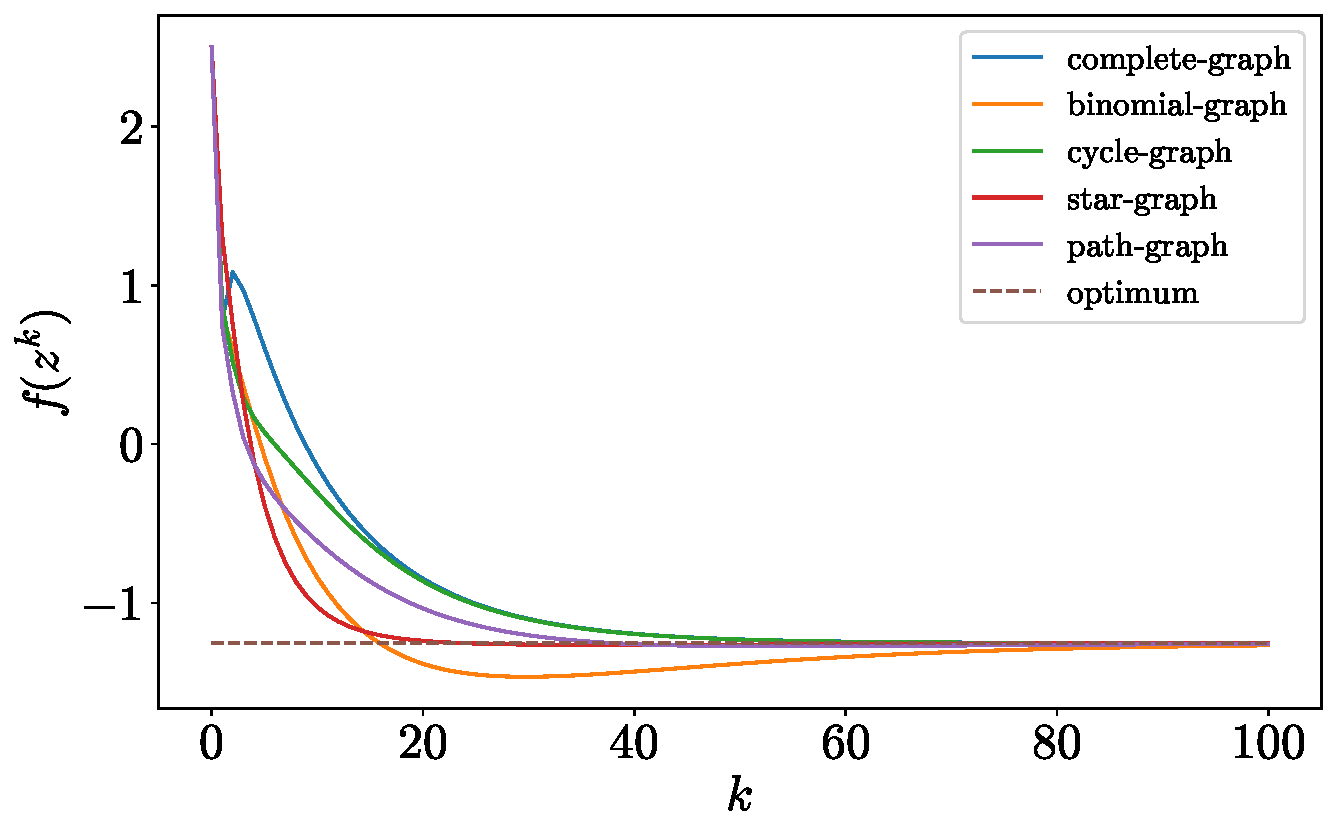
\includegraphics[width=\linewidth]{./figs/quadratic/cost_5_3_100.pdf} 
            \caption{Cost evolution}
      \end{subfigure}
      \hfill
      \begin{subfigure}[t]{0.49\textwidth}
            \centering
            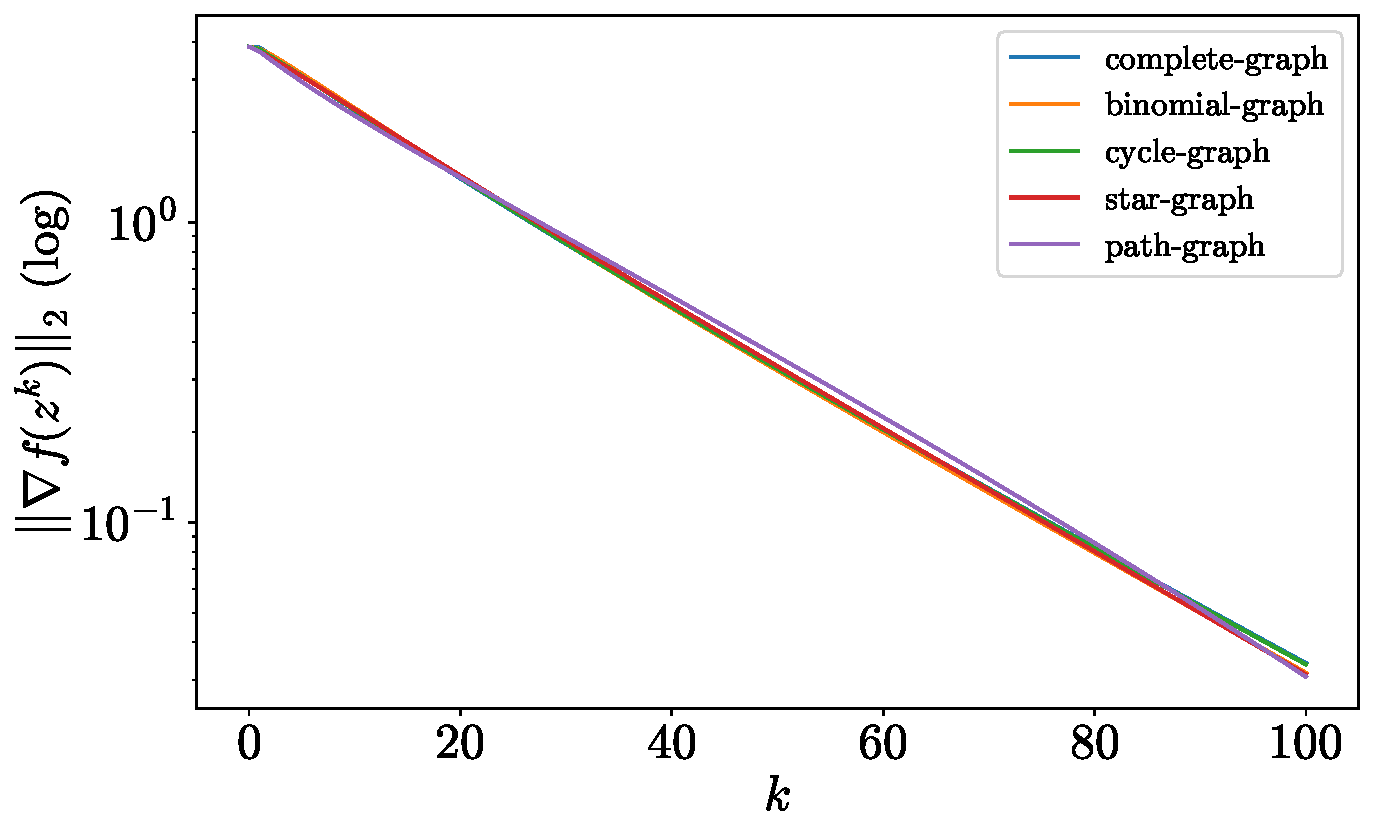
\includegraphics[width=\linewidth]{./figs/quadratic/gradient_5_3_100.pdf} 
            \caption{Gradient norm evolution}
      \end{subfigure}
      \hfill
      \begin{subfigure}[t]{0.49\textwidth}
            \centering
            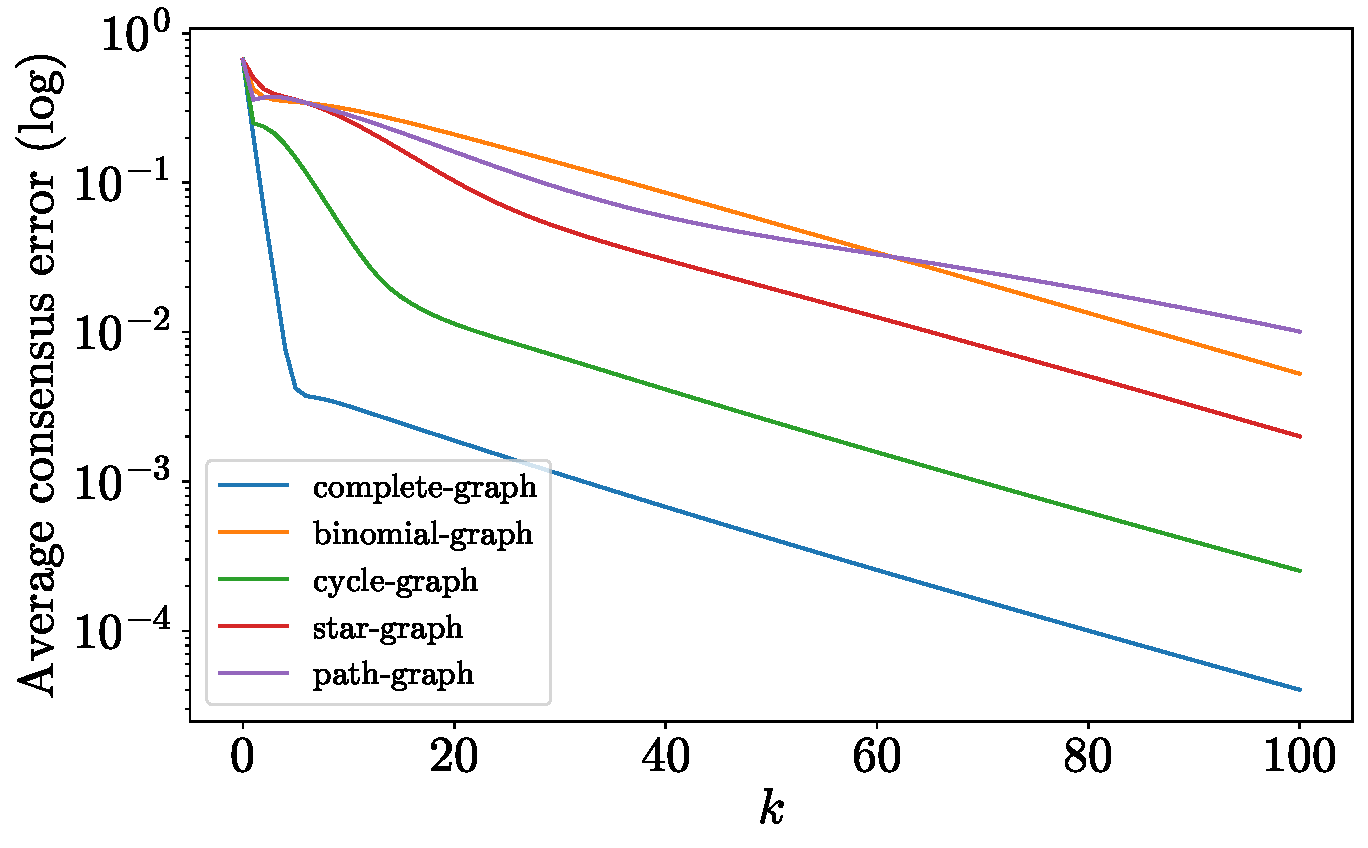
\includegraphics[width=\linewidth]{./figs/quadratic/consensus_5_3_100.pdf} 
            \caption{Consensus error}
      \end{subfigure}
      \caption{Configuration with $5$ agents in $\R^{3}$}
      \label{fig:quadratic_5_3}
\end{figure}

\begin{figure}[ht]
      \centering
      \begin{subfigure}[t]{0.49\textwidth}
            \centering
            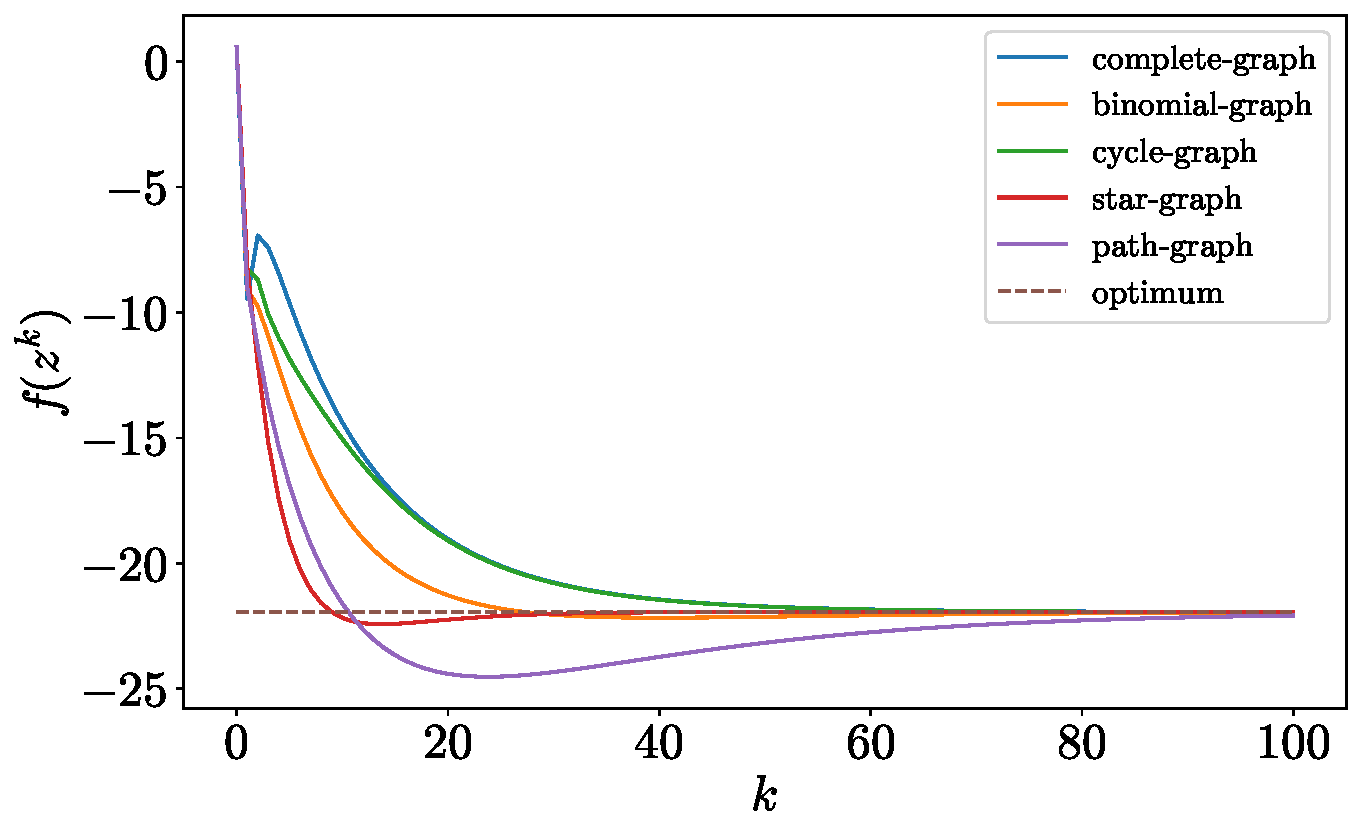
\includegraphics[width=\linewidth]{./figs/quadratic/cost_5_15_100.pdf} 
            \caption{Cost evolution}
      \end{subfigure}
      \hfill
      \begin{subfigure}[t]{0.49\textwidth}
            \centering
            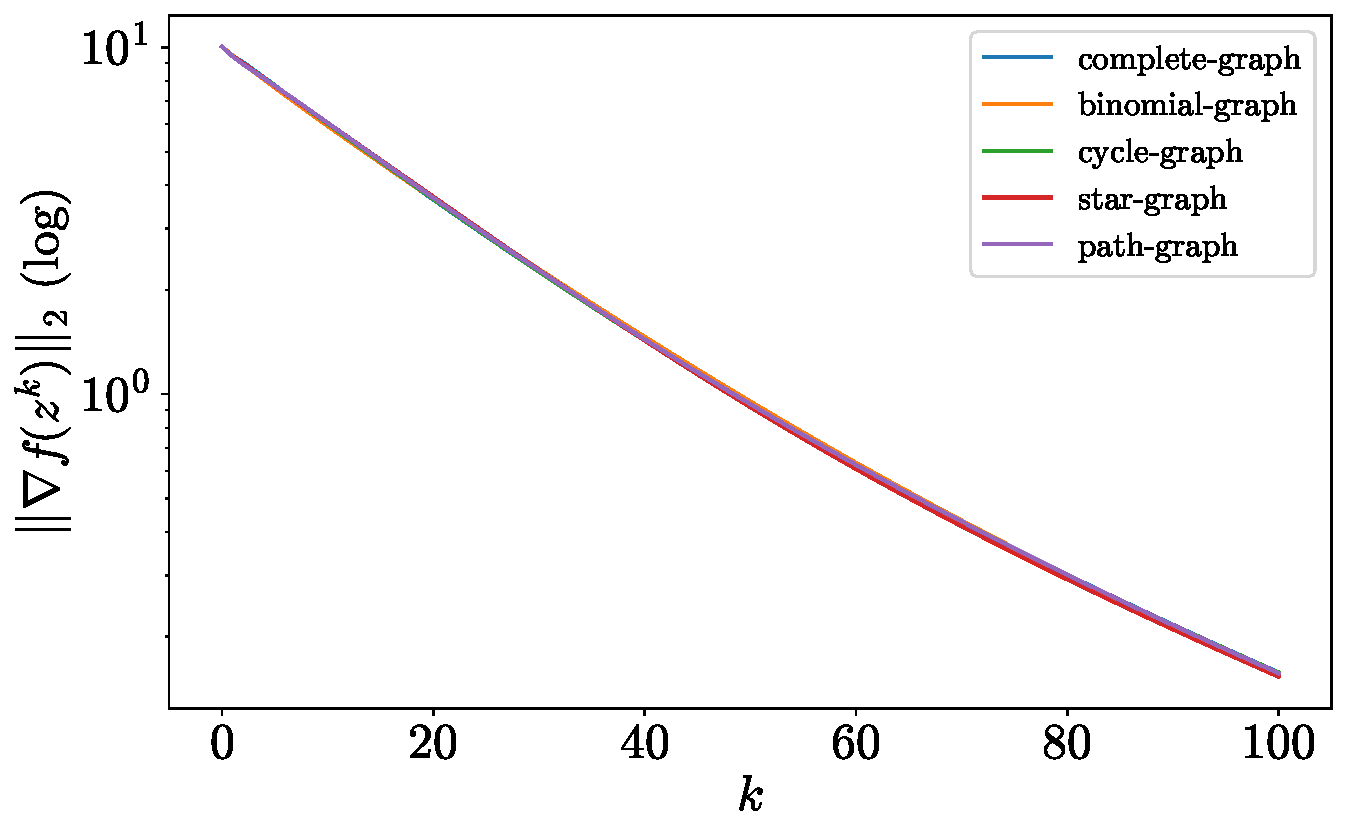
\includegraphics[width=\linewidth]{./figs/quadratic/gradient_5_15_100.pdf} 
            \caption{Gradient norm evolution}
      \end{subfigure}
      % \hfill
      % \begin{subfigure}[t]{0.49\textwidth}
      %       \centering
      %       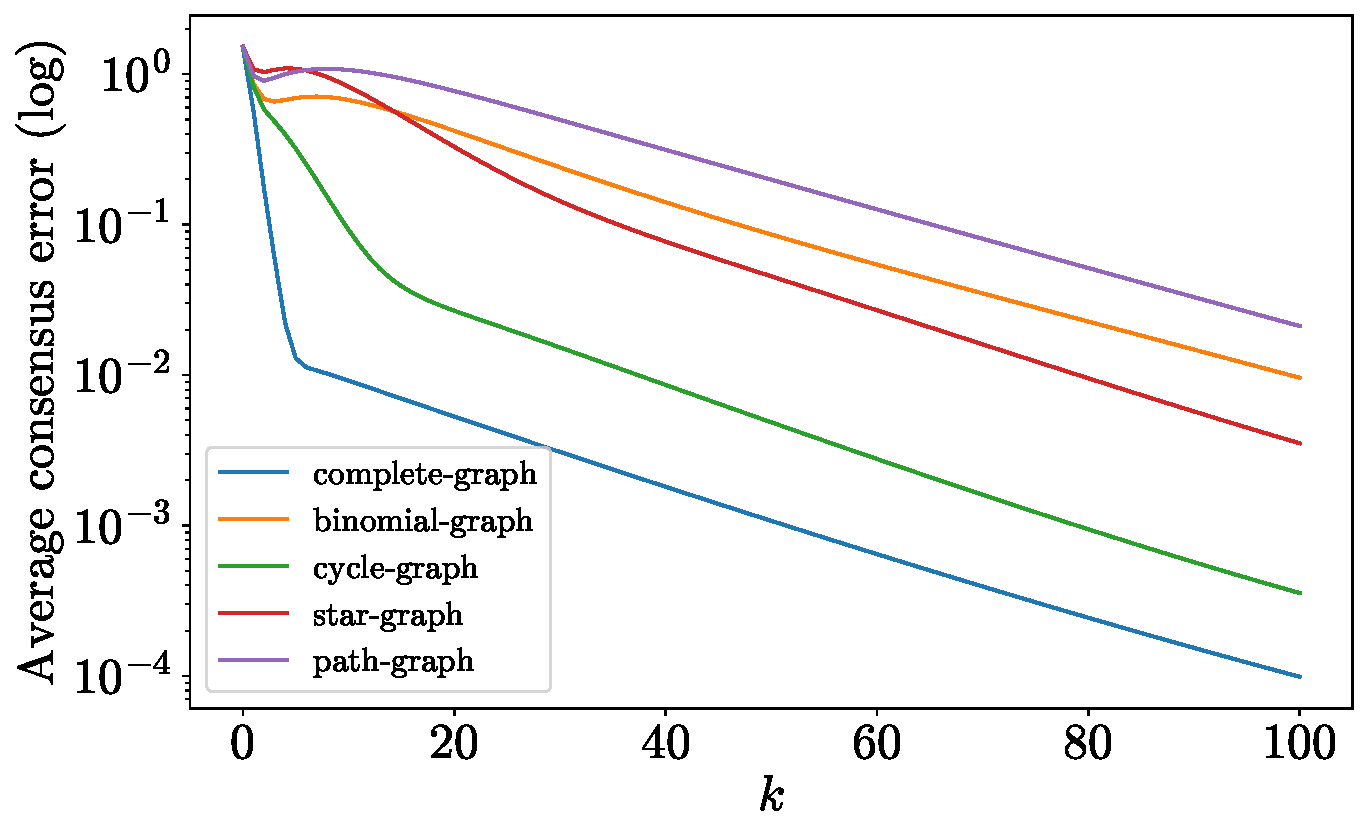
\includegraphics[width=\linewidth]{./figs/quadratic/consensus_5_15_100.pdf} 
      %       \caption{Consensus error}
      % \end{subfigure}
      \caption{Configuration with $5$ agents in $\R^{15}$}
      \label{fig:quadratic_5_15}
\end{figure}

In the case of many agents with lower dimensionality, we can observe from \Cref{fig:quadratic_15_3} that the cost function does not reach the optimum within the given number of iterations with the configurations that have a limited connectivity (e.g., path, star, and cycle graphs). Also, the gradient shows a change in terms of slope toward the end, symptom of a slower convergence. This can be explained by the fact that, by adding more agents, the overall problem includes more local losses and becomes more difficult to solve in a distributed way.

From \Cref{fig:quadratic_15_15}, we observe the same convergence behavior as in the previous case and also confirm that, with higher dimensionality, the problem is not significantly affected.


% Follo
% The following plots represent how the behavior of the algorithm changes between different kinds of networks.

% and higher dimensionality In particular, we observed a much relevant change in terms of iterations required to reach convergence for the case with 15 agents, which needed an extension in the number of iterations to show when i t
% reaches equiili

\begin{figure}[ht]
      \centering
      \begin{subfigure}[t]{0.49\textwidth}
            \centering
            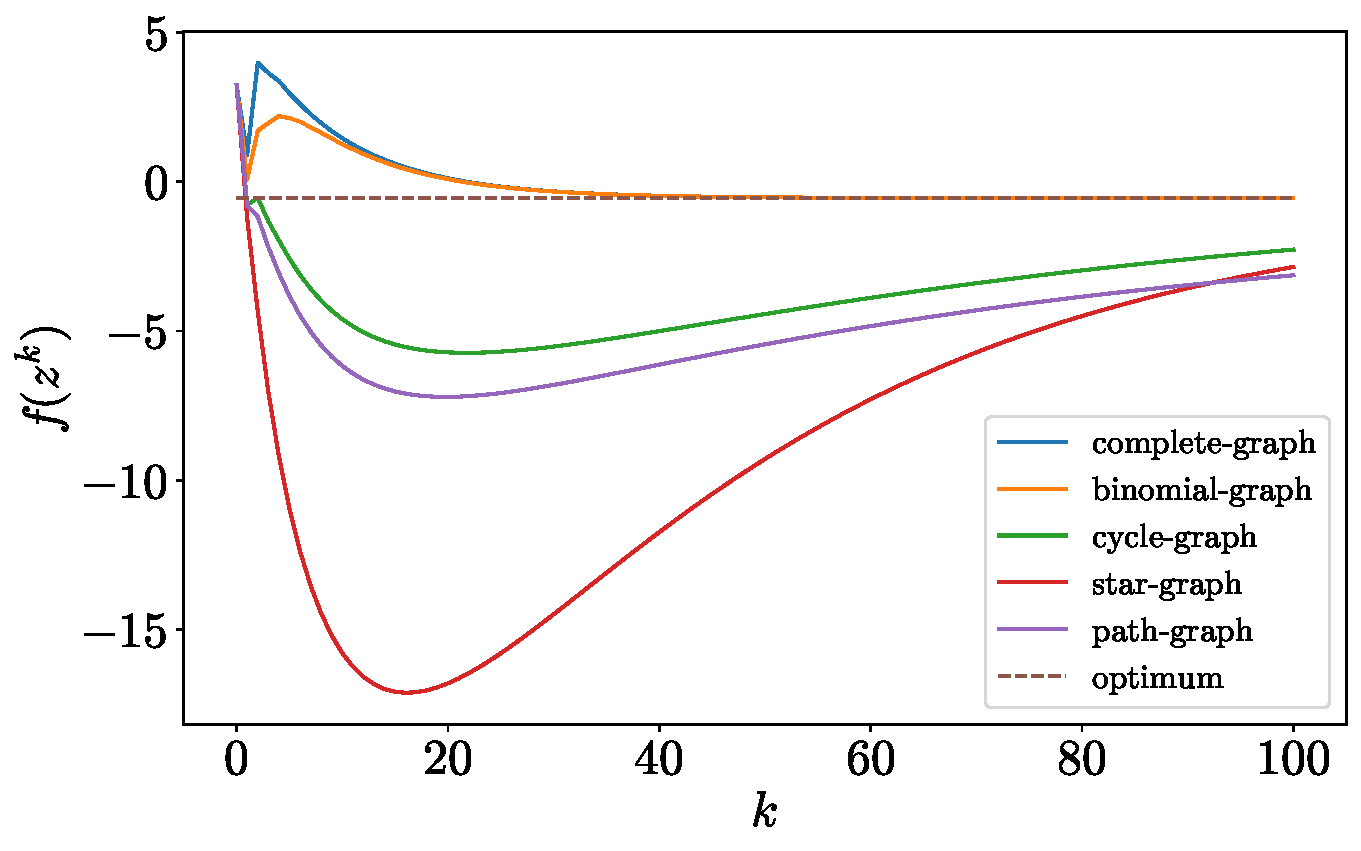
\includegraphics[width=\linewidth]{./figs/quadratic/cost_15_3_100.pdf} 
            \caption{Cost evolution}
      \end{subfigure}
      \hfill
      \begin{subfigure}[t]{0.49\textwidth}
            \centering
            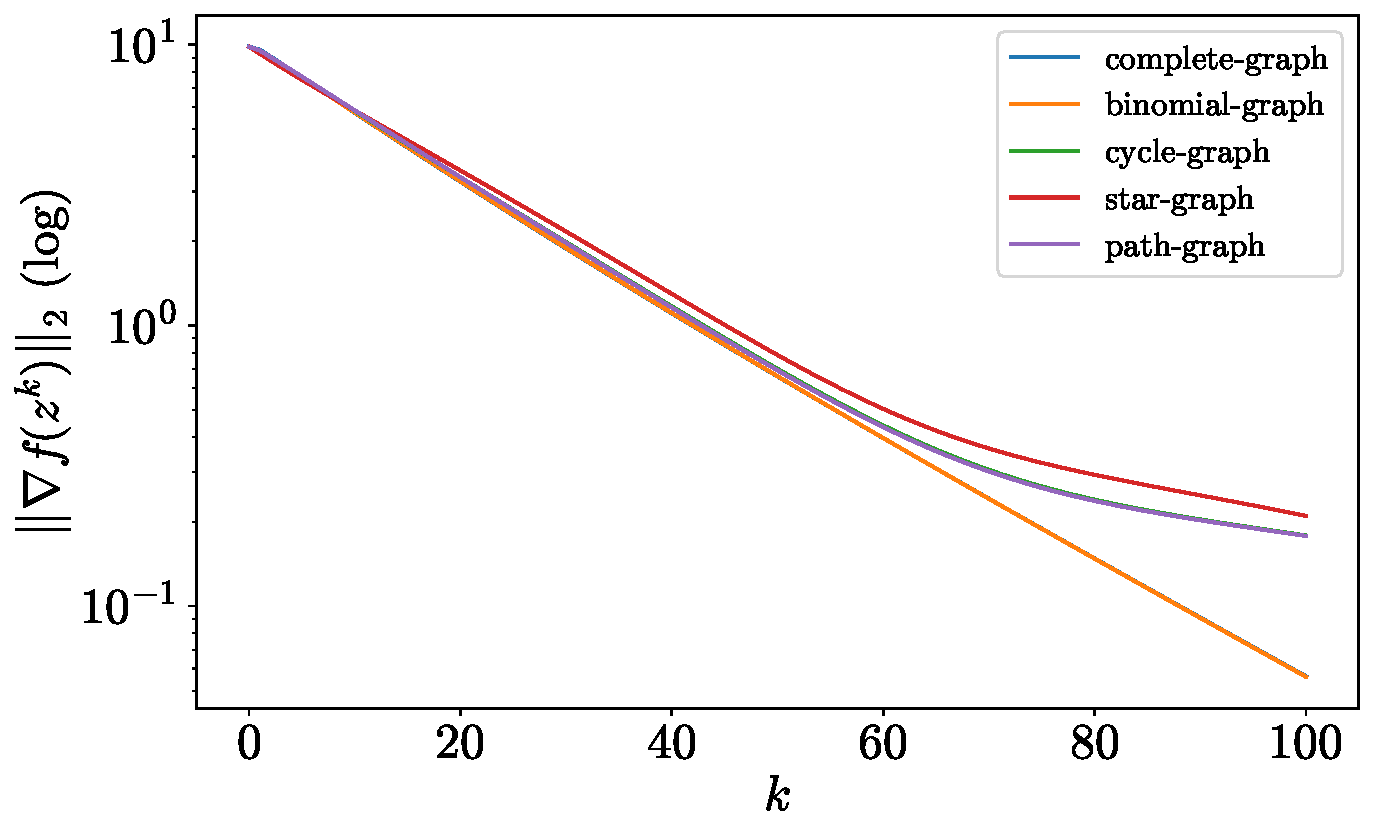
\includegraphics[width=\linewidth]{./figs/quadratic/gradient_15_3_100.pdf} 
            \caption{Gradient norm evolution}
      \end{subfigure}
      % \hfill
      % \begin{subfigure}[t]{0.49\textwidth}
      %       \centering
      %       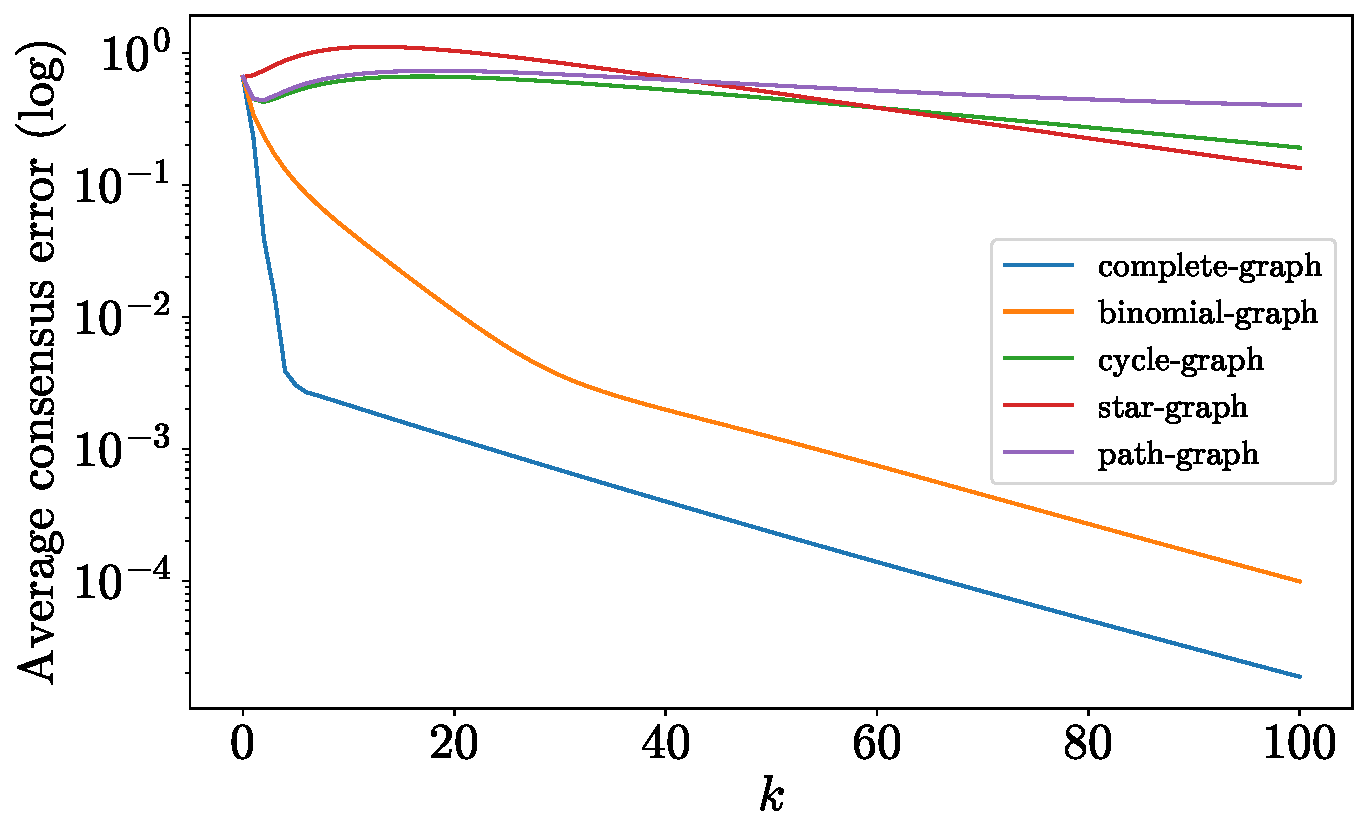
\includegraphics[width=\linewidth]{./figs/quadratic/consensus_15_3_100.pdf} 
      %       \caption{Consensus error}
      % \end{subfigure}
      \caption{Configuration with $15$ agents in $\R^{3}$}
      \label{fig:quadratic_15_3}
\end{figure}

\begin{figure}[ht]
      \centering
      \begin{subfigure}[t]{0.49\textwidth}
            \centering
            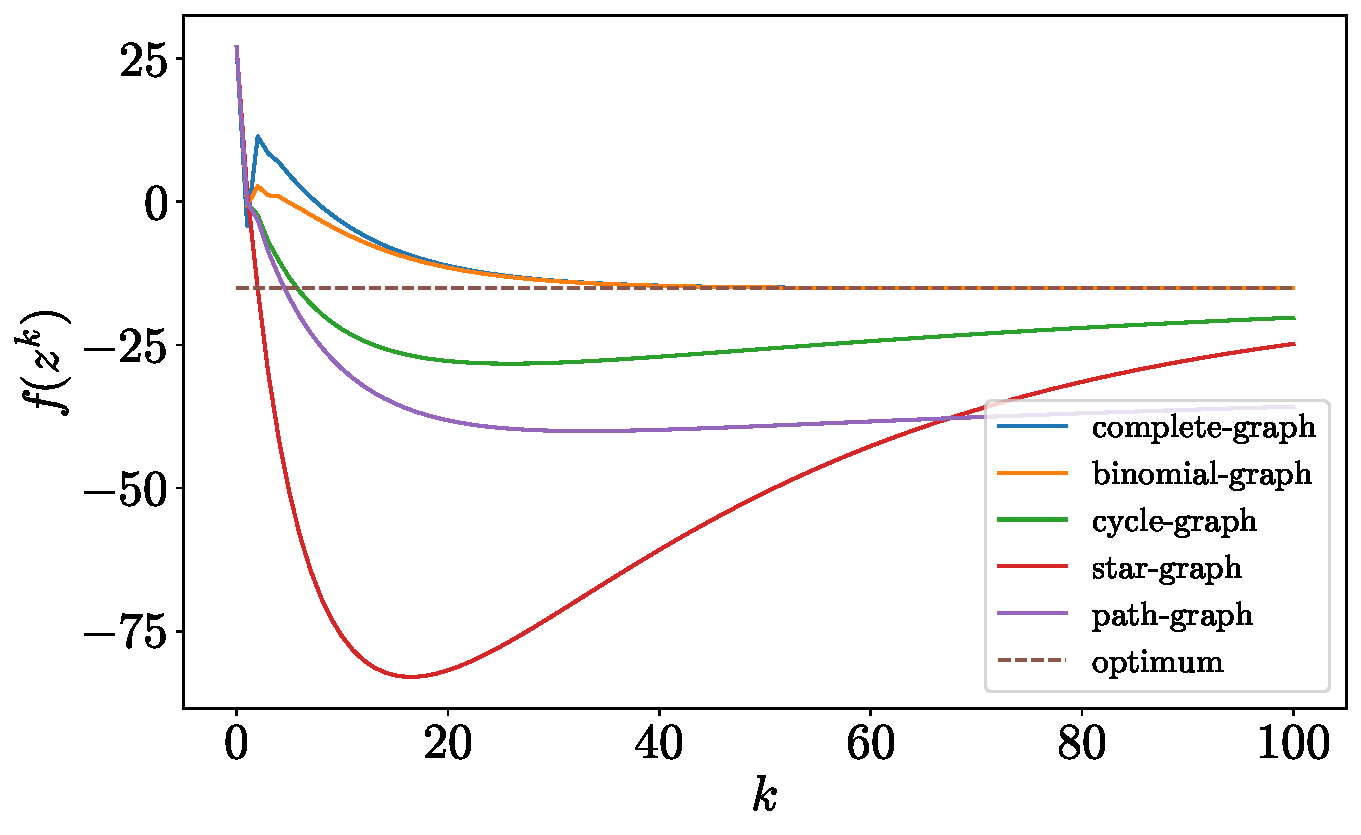
\includegraphics[width=\linewidth]{./figs/quadratic/cost_15_15_100.pdf} 
            \caption{Cost evolution}
      \end{subfigure}
      \hfill
      \begin{subfigure}[t]{0.49\textwidth}
            \centering
            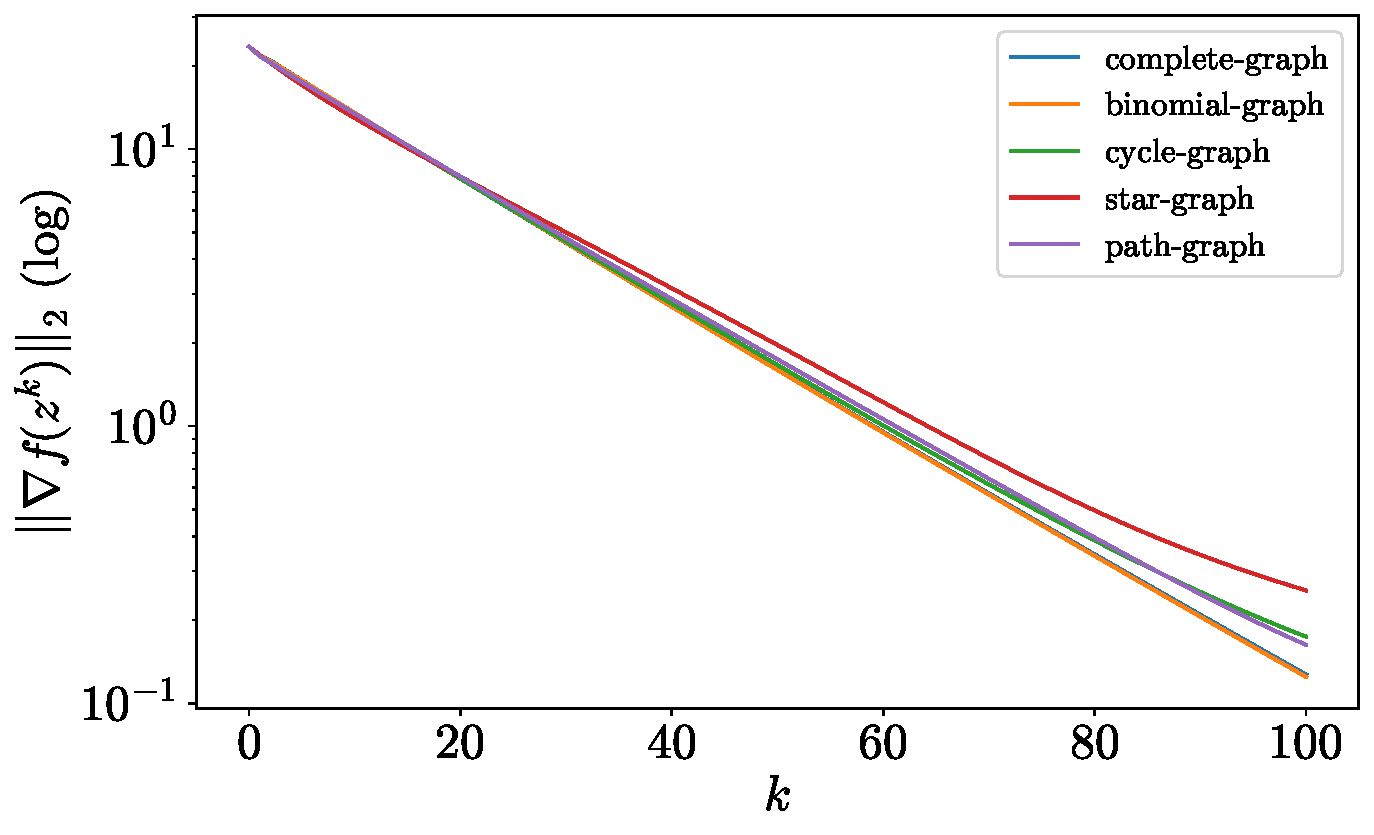
\includegraphics[width=\linewidth]{./figs/quadratic/gradient_15_15_100.pdf} 
            \caption{Gradient norm evolution}
      \end{subfigure}
      % \hfill
      % \begin{subfigure}[t]{0.49\textwidth}
      %       \centering
      %       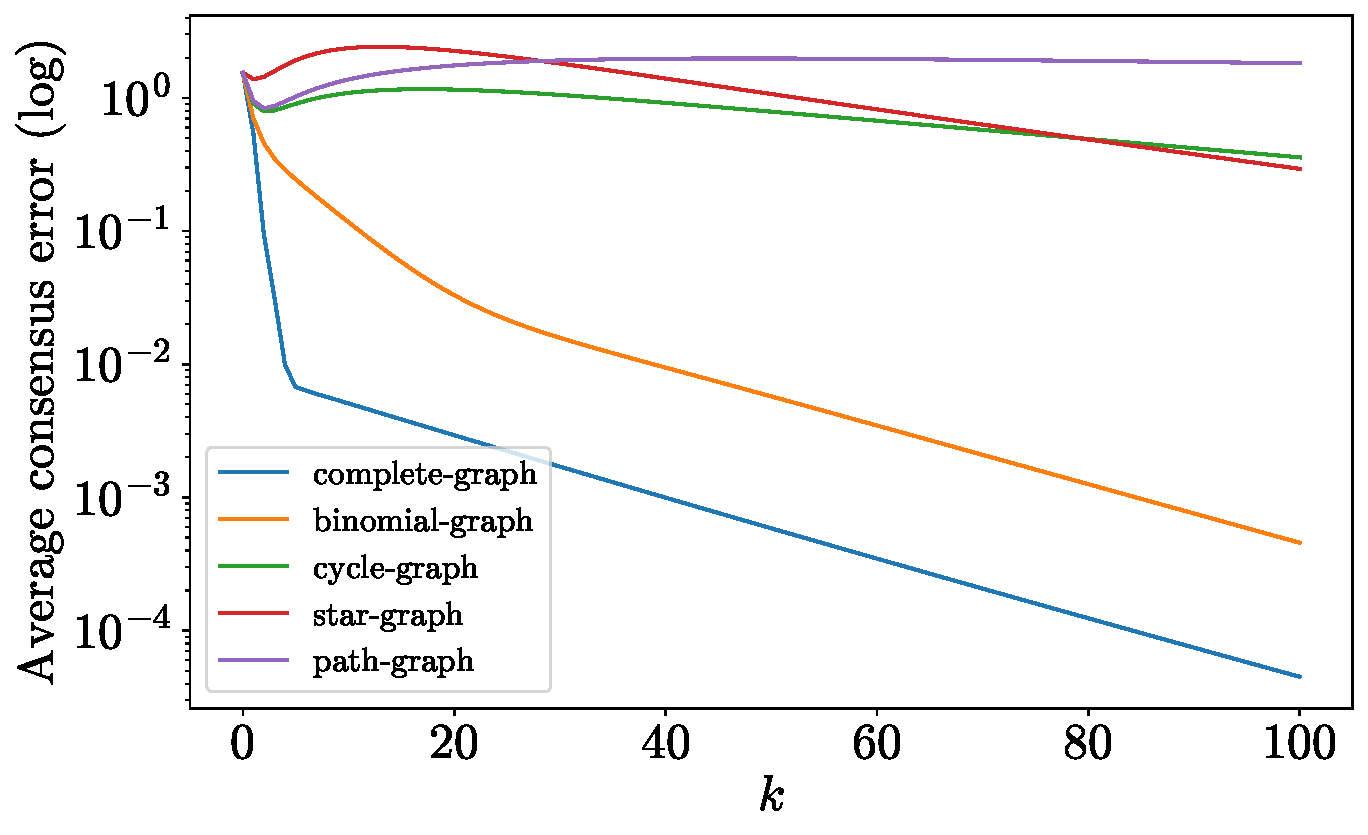
\includegraphics[width=\linewidth]{./figs/quadratic/consensus_15_15_100.pdf} 
      %       \caption{Consensus error}
      % \end{subfigure}
      \caption{Configuration with $15$ agents in $\R^{15}$}
      \label{fig:quadratic_15_15}
\end{figure}


At last, we experimented with a higher number of iterations to analyze the behavior at convergence. From \Cref{fig:quadratic_15_3_1000}, we can observe that the configuration with a complete graph is the one that converges with the most precise gradient, while the worst performing is the path graph that is converging very slowly.

\begin{figure}[ht]
      \centering
      \begin{subfigure}[t]{0.49\textwidth}
            \centering
            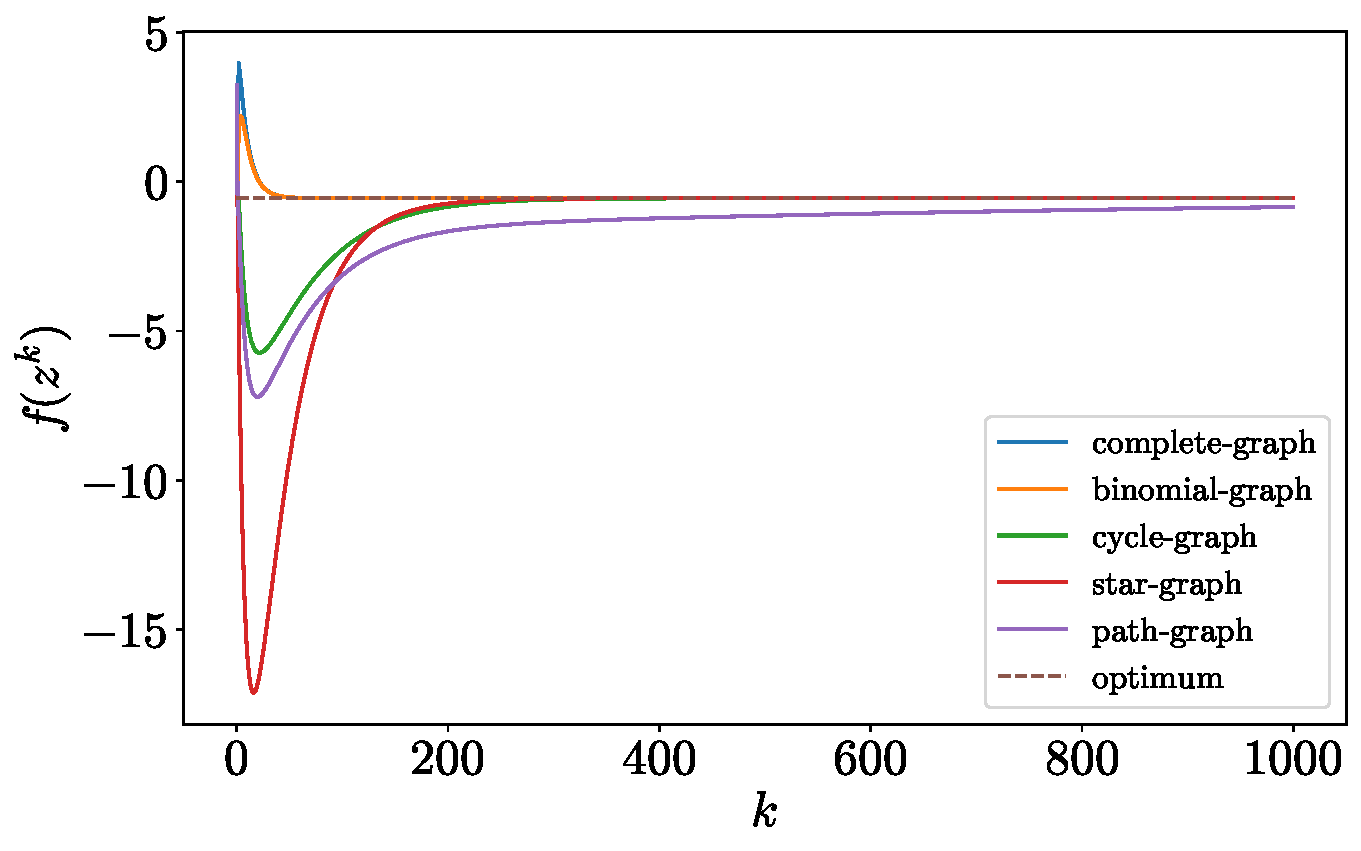
\includegraphics[width=\linewidth]{./figs/quadratic/cost_15_3_1000.pdf} 
            \caption{Cost evolution}
      \end{subfigure}
      \hfill
      \begin{subfigure}[t]{0.49\textwidth}
            \centering
            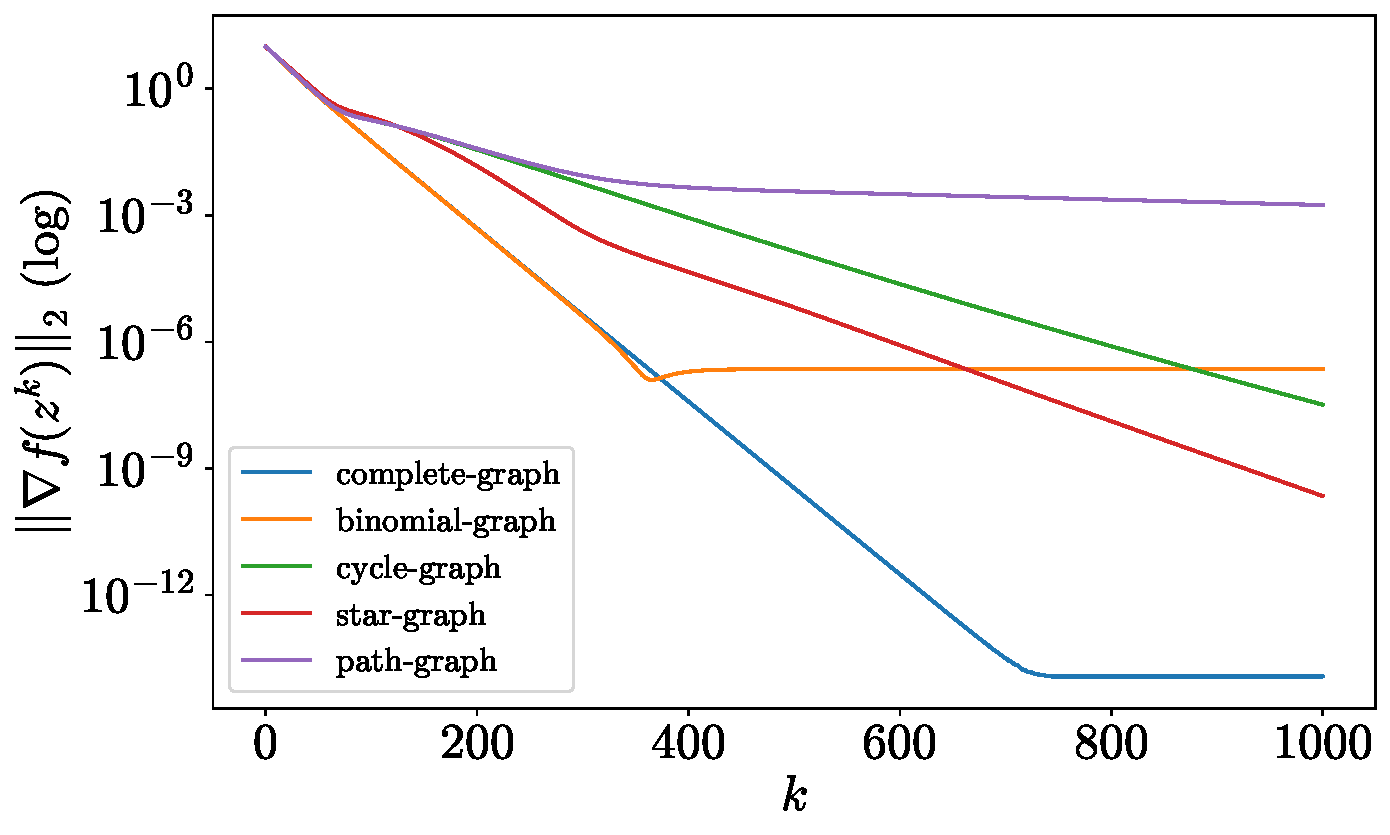
\includegraphics[width=\linewidth]{./figs/quadratic/gradient_15_3_1000.pdf} 
            \caption{Gradient norm evolution}
      \end{subfigure}
      % \hfill
      % \begin{subfigure}[t]{0.49\textwidth}
      %       \centering
      %       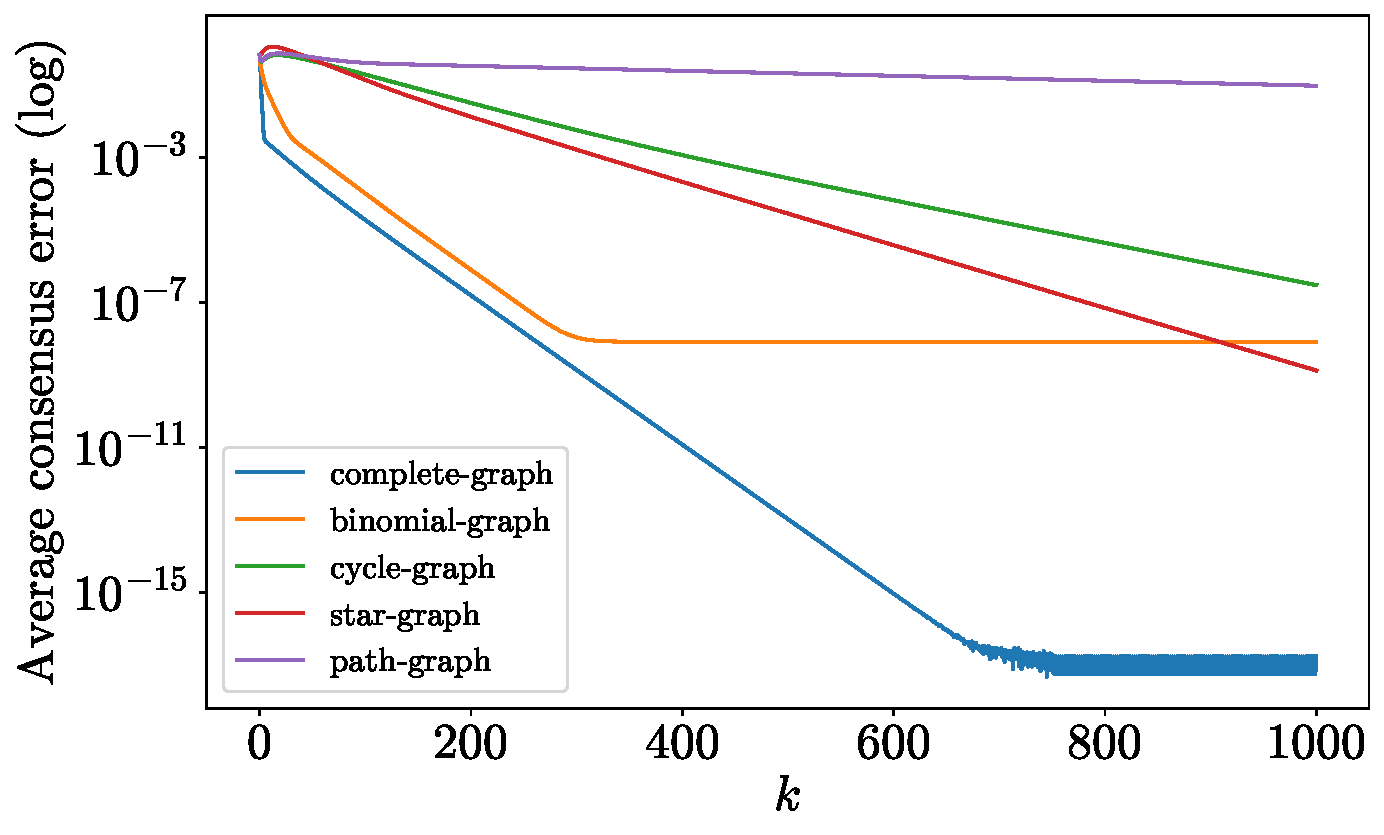
\includegraphics[width=\linewidth]{./figs/quadratic/consensus_15_3_1000.pdf} 
      %       \caption{Consensus error}
      % \end{subfigure}
      \caption{Configuration with $15$ agents in $\R^{3}$ to convergence}
      \label{fig:quadratic_15_3_1000}
\end{figure}


\subsection{Comparison with centralized gradient}

Following the previous results, we select the configuration using the complete graph for the comparison with the centralized gradient method. In \Cref{fig:quadratic_centralized_15_3}, we can observe the results with $15$ agents, but the overall behavior is the same for all configurations. It can be seen that, as one could expect, the centralized gradient method is faster to converge compared to a distributed algorithm as it has available all the global information and does not rely on information exchange with the neighbors.

\begin{figure}[ht]
      \centering
      \begin{subfigure}[t]{0.49\textwidth}
            \centering
            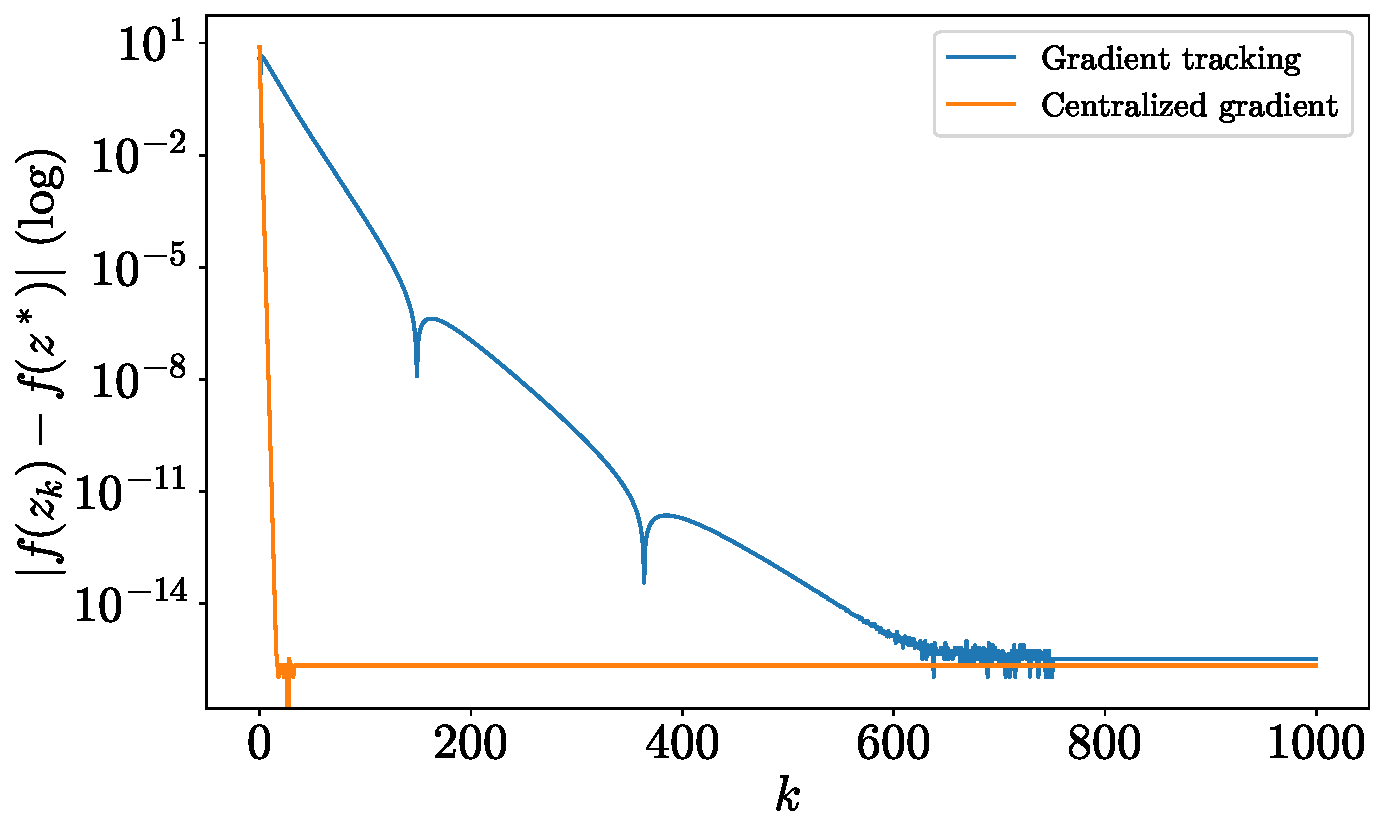
\includegraphics[width=\linewidth]{./figs/quadratic/distance_centralized_15_3_1000.pdf} 
            \caption{Distance to optimum}
      \end{subfigure}
      \hfill
      \begin{subfigure}[t]{0.49\textwidth}
            \centering
            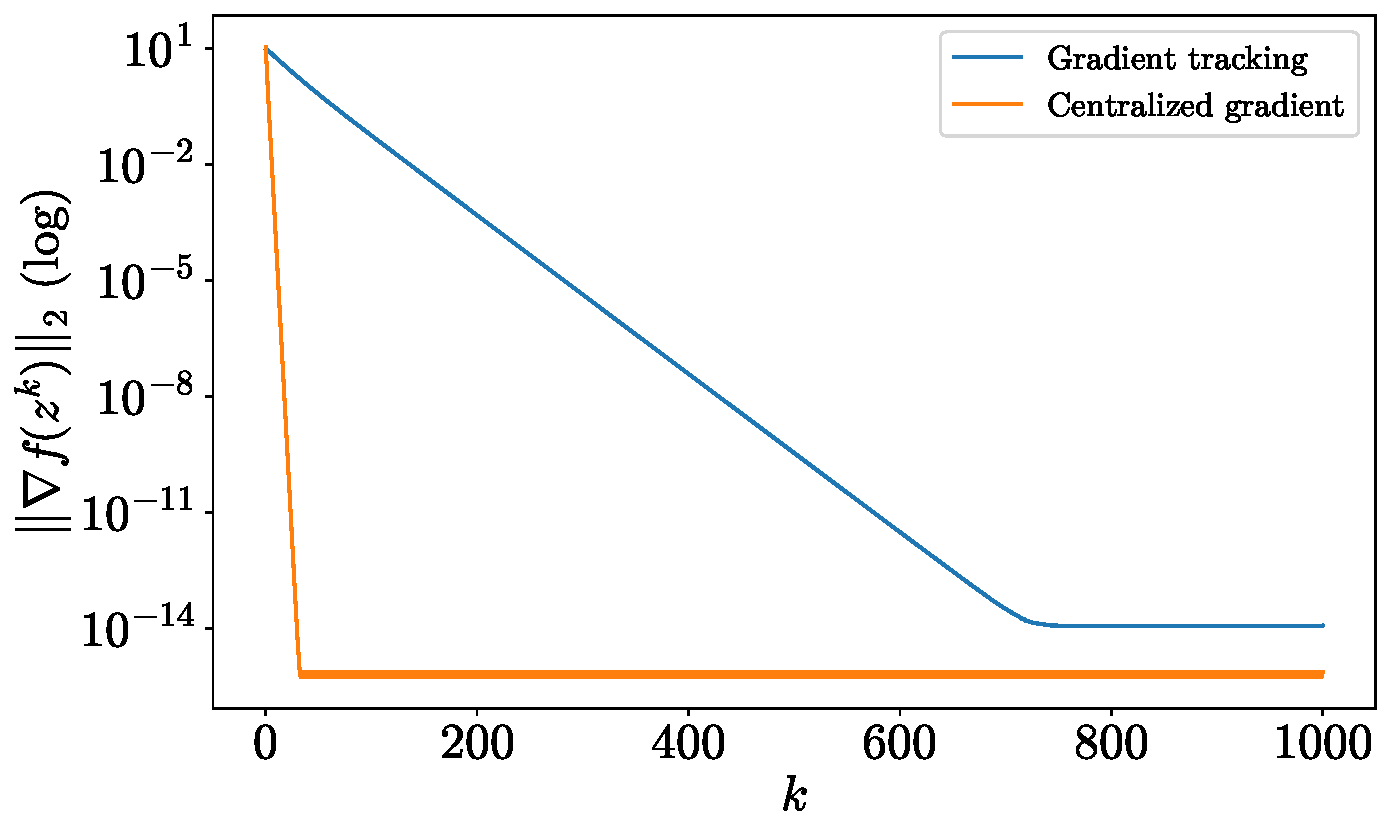
\includegraphics[width=\linewidth]{./figs/quadratic/gradient_centralized_15_3_1000.pdf} 
            \caption{Gradient norm evolution}
      \end{subfigure}
      \caption{Configuration with $15$ agents in $\R^{3}$ compared to centralized gradient}
      \label{fig:quadratic_centralized_15_3}
\end{figure}



\section{Cooperative multi-robot target localization}

The second part of the task involves applying the gradient tracking algorithm for estimating the position of $N_T$ fixed targets in a distributed way through $N_R$ tracking robots. Each robot is located at position $\p_i \in \R^2$ and it is assumed that the distance measured from each robot is noisy. Given the position of the robot $\p_i$ and of the target $\p_\tau$, we model the measured noisy distance $d_{i,\tau}$ as follows:
\[
      d_{i,\tau} = \Vert \p_i - \p_\tau \Vert + \varepsilon \cdot \texttt{noise}
\]
where $\texttt{noise}$ is drawn from some distribution and $\varepsilon$ is the noise rate.

The local loss each robot $i$ uses is the following:
\[
      \begin{gathered}
            l_i(\z) = \sum_{\tau=1}^{N_T} \left( d_{i,\tau}^2 - \Vert \z_{\tau} - \p_i \Vert^2 \right)^2
            \quad
            \nabla l_{i}(\z) = (\nabla l_{i,1}(\z_{1}), \dots, \nabla l_{i,N_T}(\z_{N_T}))
            \\
            \nabla l_{i,j}(\z_{j}) = -4 \left( d_{i,j}^2 - \Vert \z_{j} - \p_i \Vert^2 \right) \left( \z_{j} - \p_i \right)
      \end{gathered}
\]
where $\z = (\z_{\tau_1}, \dots, \z_{\tau_{N_T}}) \in \R^{2N_T}$ is the stack of decision variables of robot $i$ containing the estimated positions of the targets $\z_{\tau} \in \R^2$ and $\nabla l_i(\z) \in \R^{2N_T}$ is the concatenation of the gradients computed at each target.

We approach the experimentation of such algorithm by trying different graph patterns and comparing with the centralized gradient method, similarly to the previous case. At first, we evaluated the performance of the algorithm in the following cases, all with the same type of noise:
\begin{itemize}
      \item Network of 5 robots and 1 target,
      \item Network of 5 robots and 3 targets, and
      \item Network of 15 robots and 3 targets.
\end{itemize}

Then, the focus switched to observe how much the performance changes in terms of noise. By fixing the problem configuration, we experimented with varying Gaussian noises, Poisson noises and noise rates.


\subsection{Comparison between different graph patterns}

In terms of graph pattern, we can observe from \Cref{fig:tracking_5_1} and \Cref{fig:tracking_5_3} that with the same number of robots and increasing number of targets, the number of iterations required to converge is the same. This makes sense as each target is independent of the others.

\begin{figure}[ht]
      \centering
      \begin{subfigure}[t]{0.49\textwidth}
            \centering
            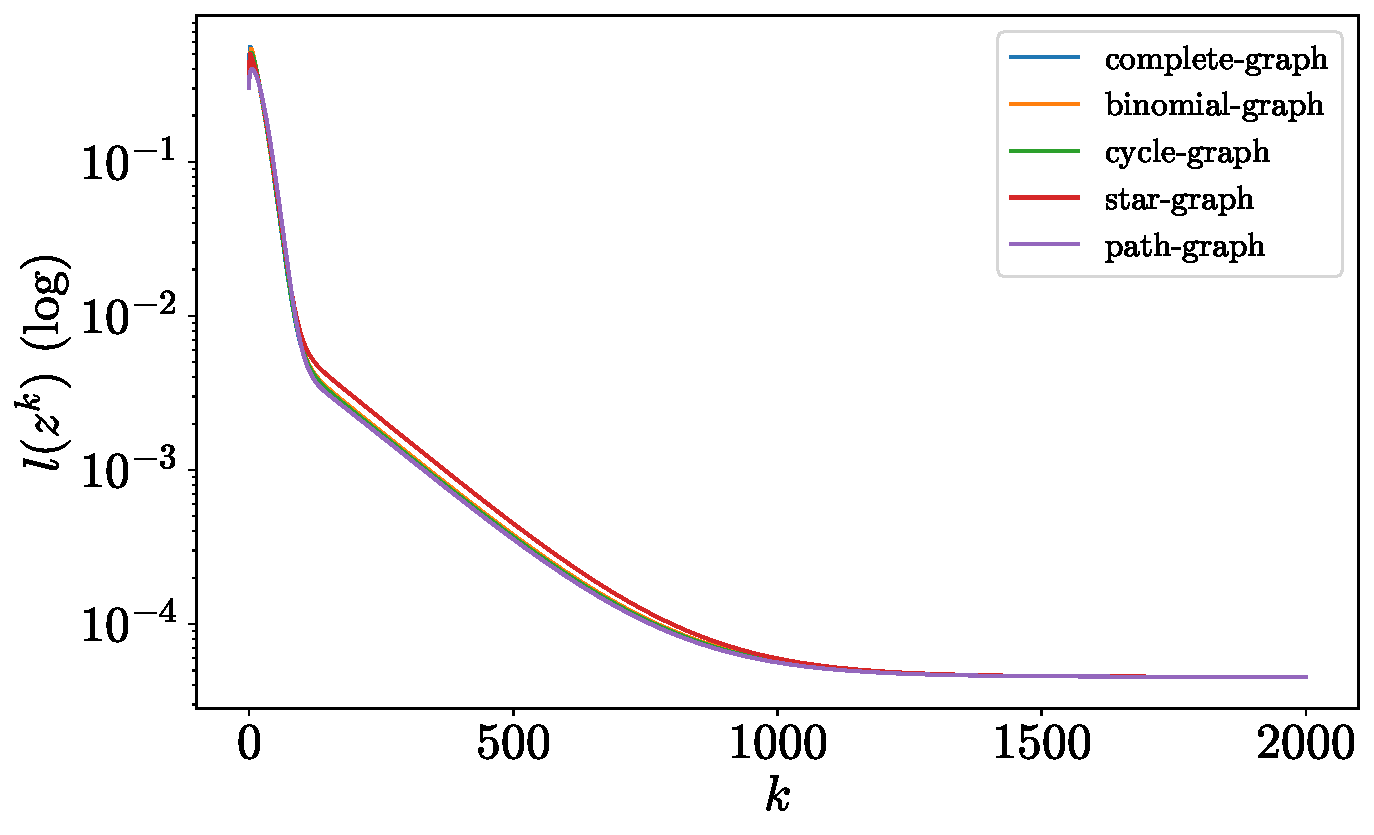
\includegraphics[width=\linewidth]{./figs/tracking/loss_5_1_2_2000.pdf} 
            \caption{Loss evolution}
      \end{subfigure}
      \hfill
      \begin{subfigure}[t]{0.49\textwidth}
            \centering
            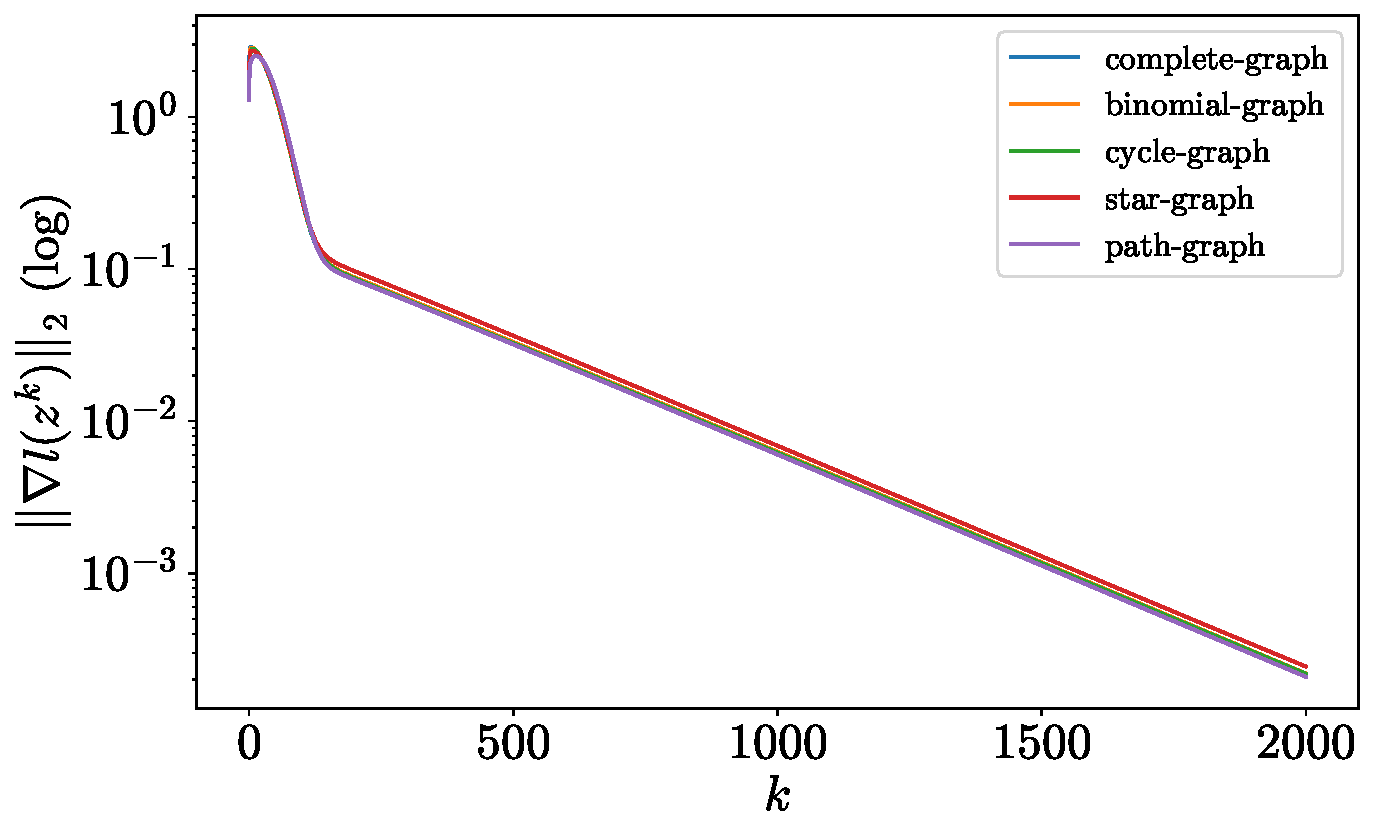
\includegraphics[width=\linewidth]{./figs/tracking/gradient_5_1_2_2000.pdf} 
            \caption{Gradient norm evolution}
      \end{subfigure}
      \caption{Configuration with $5$ robots and $1$ target}
      \label{fig:tracking_5_1}
\end{figure}

\begin{figure}[ht]
      \centering
      \begin{subfigure}[t]{0.49\textwidth}
            \centering
            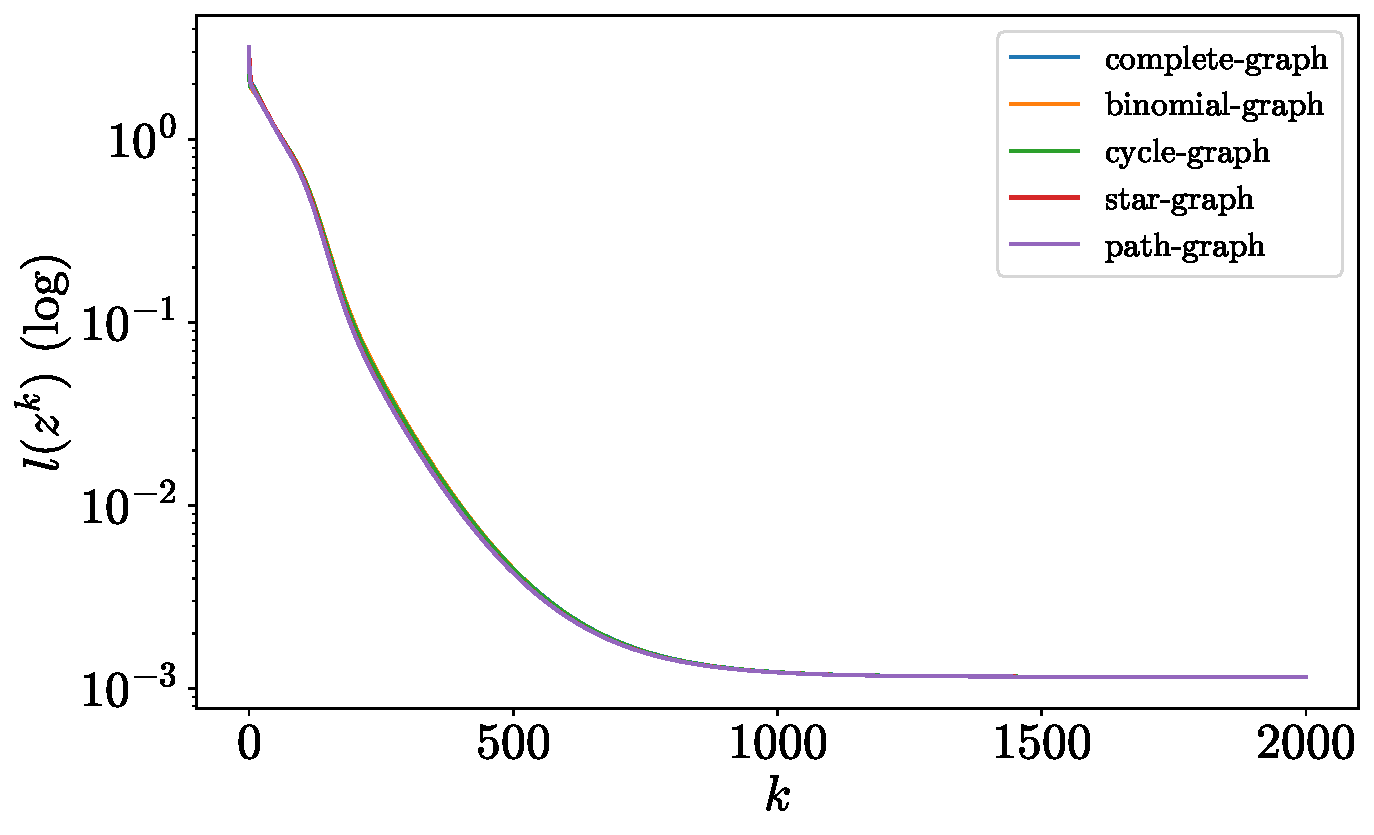
\includegraphics[width=\linewidth]{./figs/tracking/loss_5_3_2_2000.pdf} 
            \caption{Loss evolution}
      \end{subfigure}
      \hfill
      \begin{subfigure}[t]{0.49\textwidth}
            \centering
            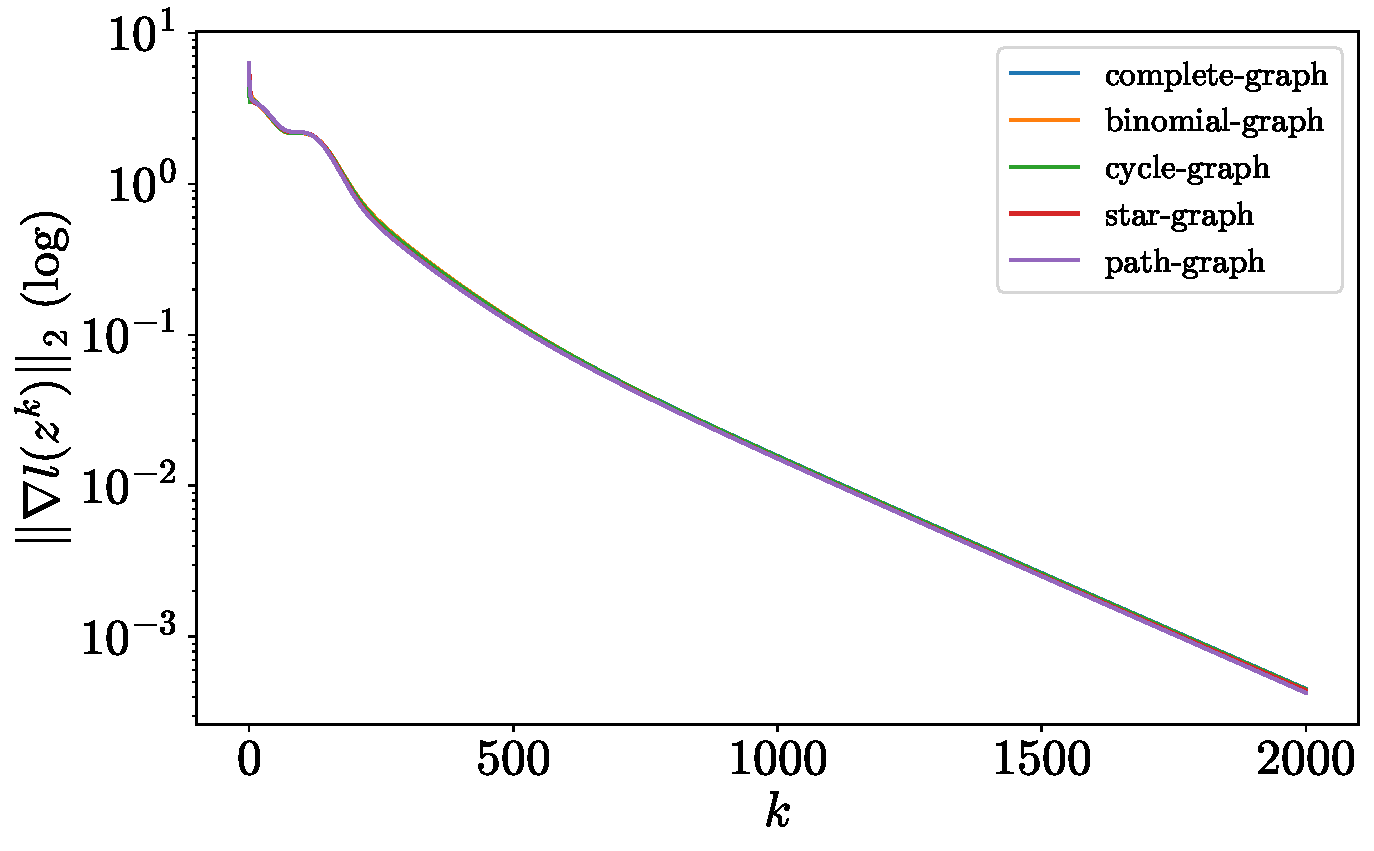
\includegraphics[width=\linewidth]{./figs/tracking/gradient_5_3_2_2000.pdf} 
            \caption{Gradient norm evolution}
      \end{subfigure}
      \caption{Configuration with $5$ robots and $3$ targets}
      \label{fig:tracking_5_3}
\end{figure}

Instead, by increasing the number of tracking robots, we can see from \Cref{fig:tracking_15_3} that the plateau is reached in fewer number of iteration, which intuitively means that more tracking robots help in reaching a faster convergence.

\begin{figure}[ht]
      \centering
      \begin{subfigure}[t]{0.49\textwidth}
            \centering
            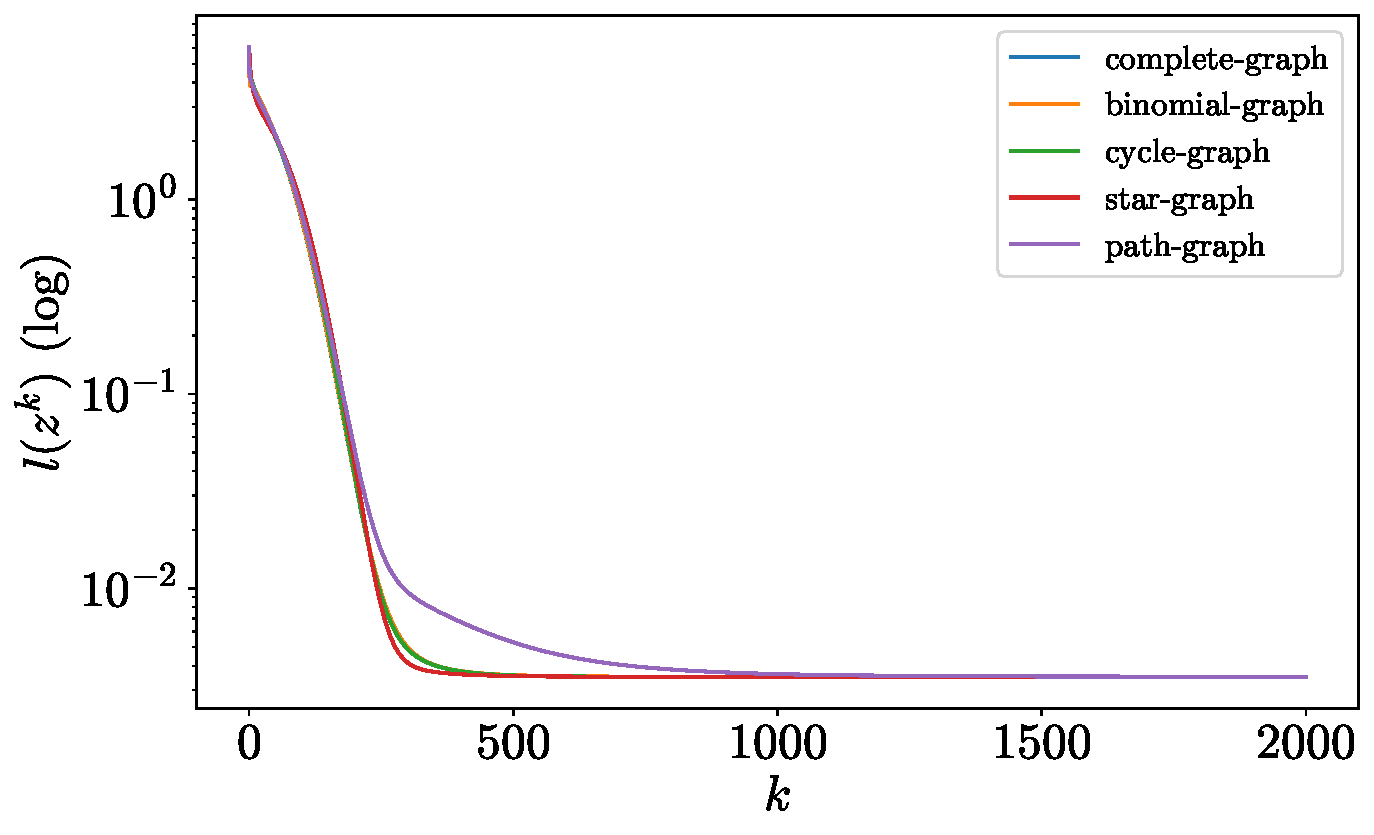
\includegraphics[width=\linewidth]{./figs/tracking/loss_15_3_2_2000.pdf} 
            \caption{Loss evolution}
      \end{subfigure}
      \hfill
      \begin{subfigure}[t]{0.49\textwidth}
            \centering
            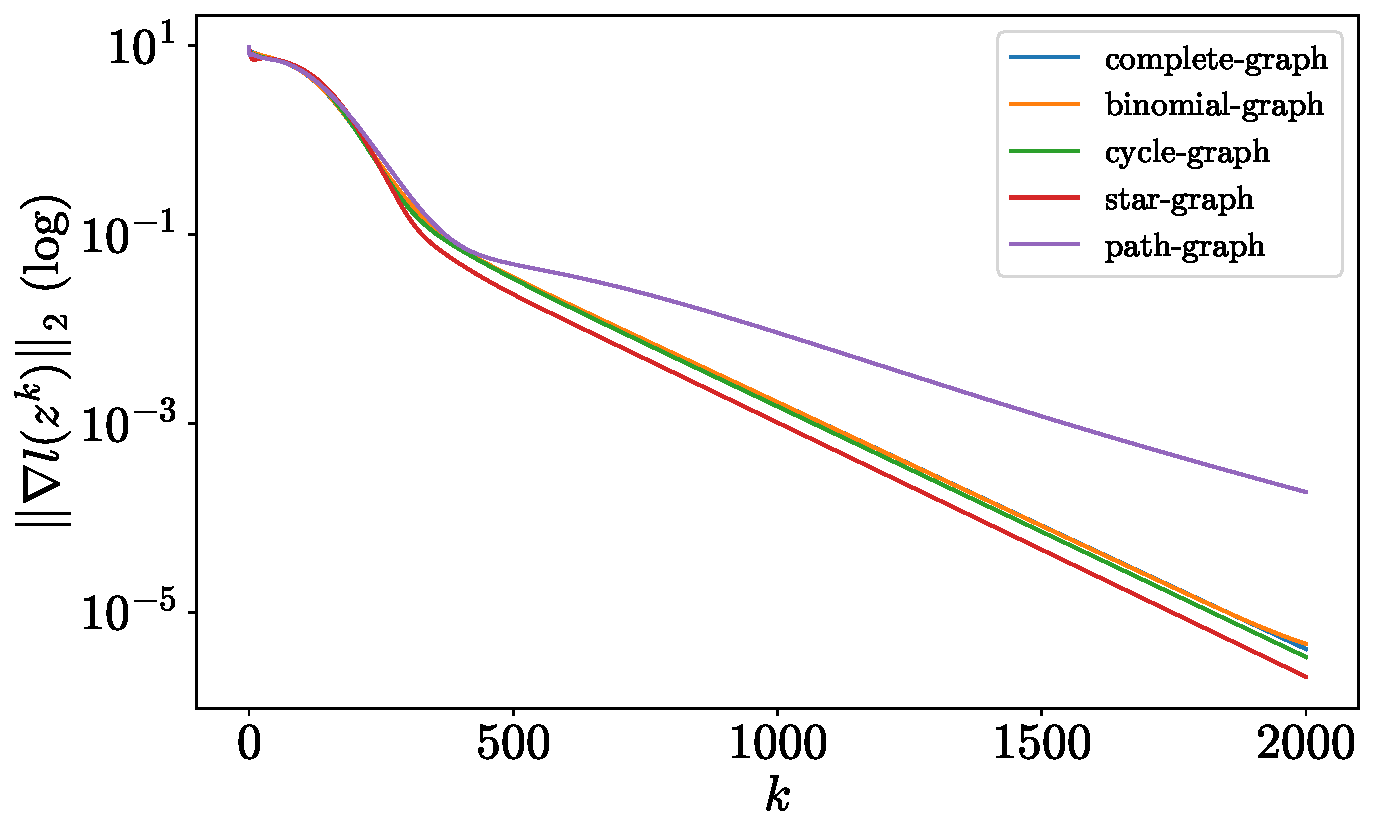
\includegraphics[width=\linewidth]{./figs/tracking/gradient_15_3_2_2000.pdf} 
            \caption{Gradient norm evolution}
      \end{subfigure}
      \caption{Configuration with $15$ robots and $3$ targets}
      \label{fig:tracking_15_3}
\end{figure}

Moreover, as the total loss is a summation, we must note that the overall loss is higher in the case of more agent, but this does not indicate worse tracking results. We report in \Cref{tab:tracking_error} the average distance between the estimated and real target positions for the three configurations we discussed. It can be seen that, consistently with the behavior of the loss, all graph patterns converge to roughly the same average error. Furthermore, as we mentioned, with more robots the average tracking error is lower even with a loss that has a higher magnitude.

\begin{table}[ht]
      \centering
      \small
      \caption{Average tracking error at the last iteration}
      \label{tab:tracking_error}
      \begin{tabular}{lccc}
            \toprule
            & $N_R=5, N_T=1$ & $N_R=5, N_T=3$ & $N_R=15, N_T=3$ \\
            \midrule
            \textbf{Complete} & $0.03008$ & $0.00554$ & $0.00500$ \\
            \textbf{Binomial} & $0.03008$ & $0.00554$ & $0.00500$ \\
            \textbf{Cycle}    & $0.03008$ & $0.00554$ & $0.00500$ \\
            \textbf{Star}     & $0.03007$ & $0.00554$ & $0.00500$ \\
            \textbf{Path}     & $0.03009$ & $0.00553$ & $0.00501$ \\
            \bottomrule
      \end{tabular}
\end{table}


\subsection{Comparison with centralized gradient}

Compared with the centralized gradient algorithm, the plots in \Cref{fig:tracking_centralized_5_3} confirm what we observed before in the case of quadratic functions. The convergence speed is faster and more accurate in a centralized approach, which also results in a lower average tracking error.

\begin{figure}[ht]
      \centering
      \begin{subfigure}[t]{0.49\textwidth}
            \centering
            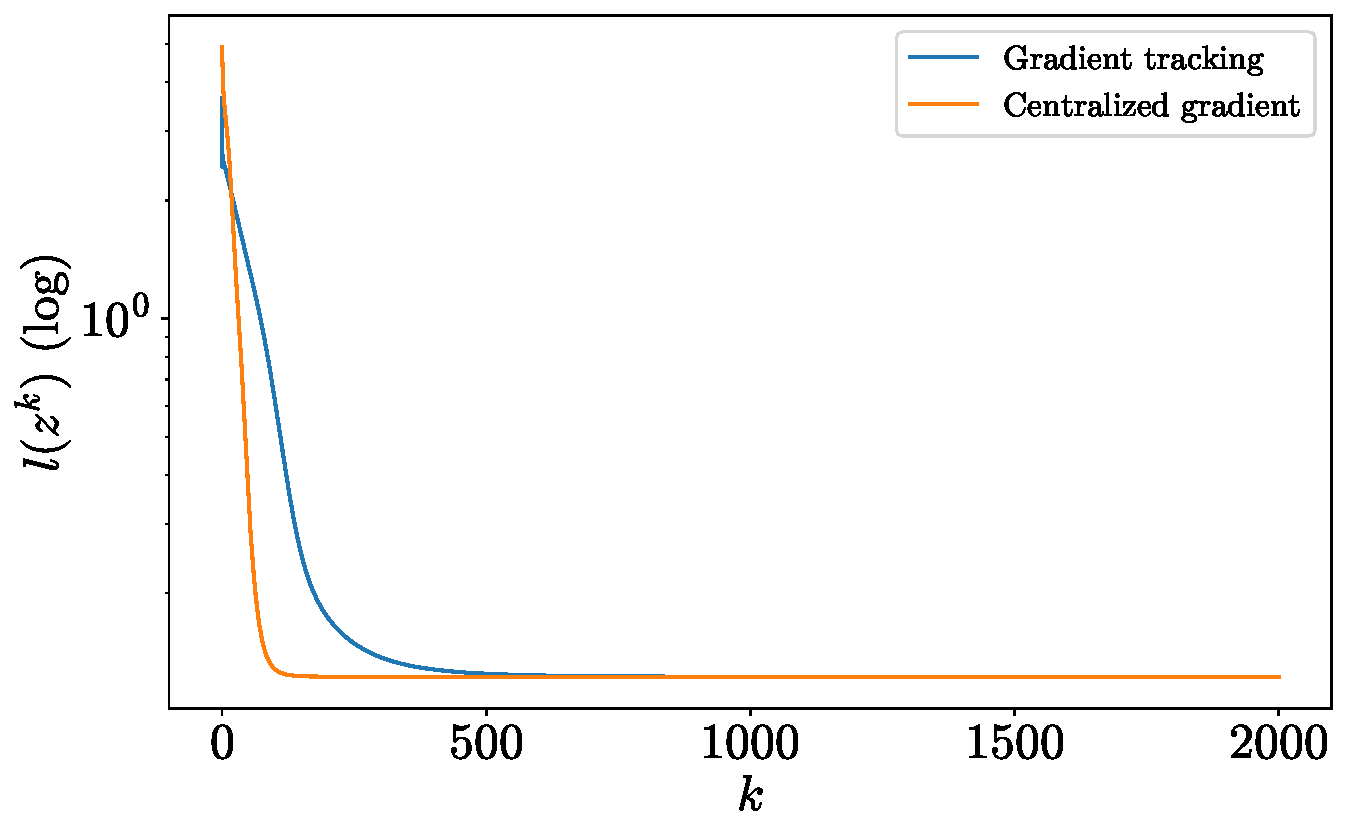
\includegraphics[width=\linewidth]{./figs/tracking/loss_centralized_5_3_2_2000.pdf} 
            \caption{Loss evolution}
      \end{subfigure}
      \hfill
      \begin{subfigure}[t]{0.49\textwidth}
            \centering
            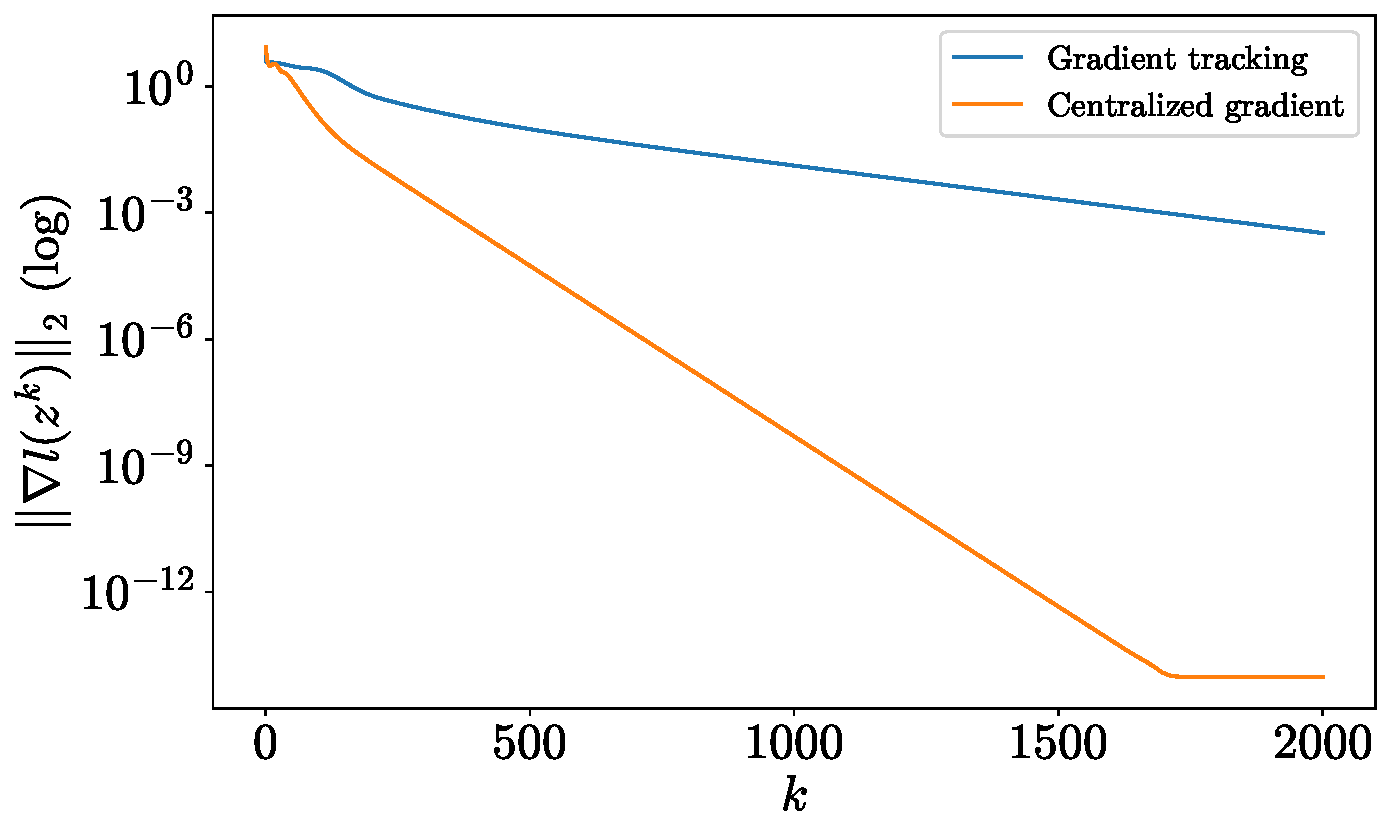
\includegraphics[width=\linewidth]{./figs/tracking/gradient_centralized_5_3_2_2000.pdf} 
            \caption{Gradient norm evolution}
      \end{subfigure}
      \caption{Configuration with $5$ robots and $3$ targets with centralized gradient}
      \label{fig:tracking_centralized_5_3}
\end{figure}


\subsection{Different noises}

From the experiments with different noises, we observed a worsening in performance that is proportional to the amount of noise injected into the distance measurement, implying as one could expect that more noise leads to worse results. This behavior is consistent with noise drawn from different distributions as in \Cref{fig:tracking_gaussian_15_3} and \Cref{fig:tracking_poisson_15_3}, and also when the noise rate is increased as in \Cref{fig:tracking_rates_15_3}.

\begin{figure}[ht]
      \centering
      \begin{subfigure}[t]{0.49\textwidth}
            \centering
            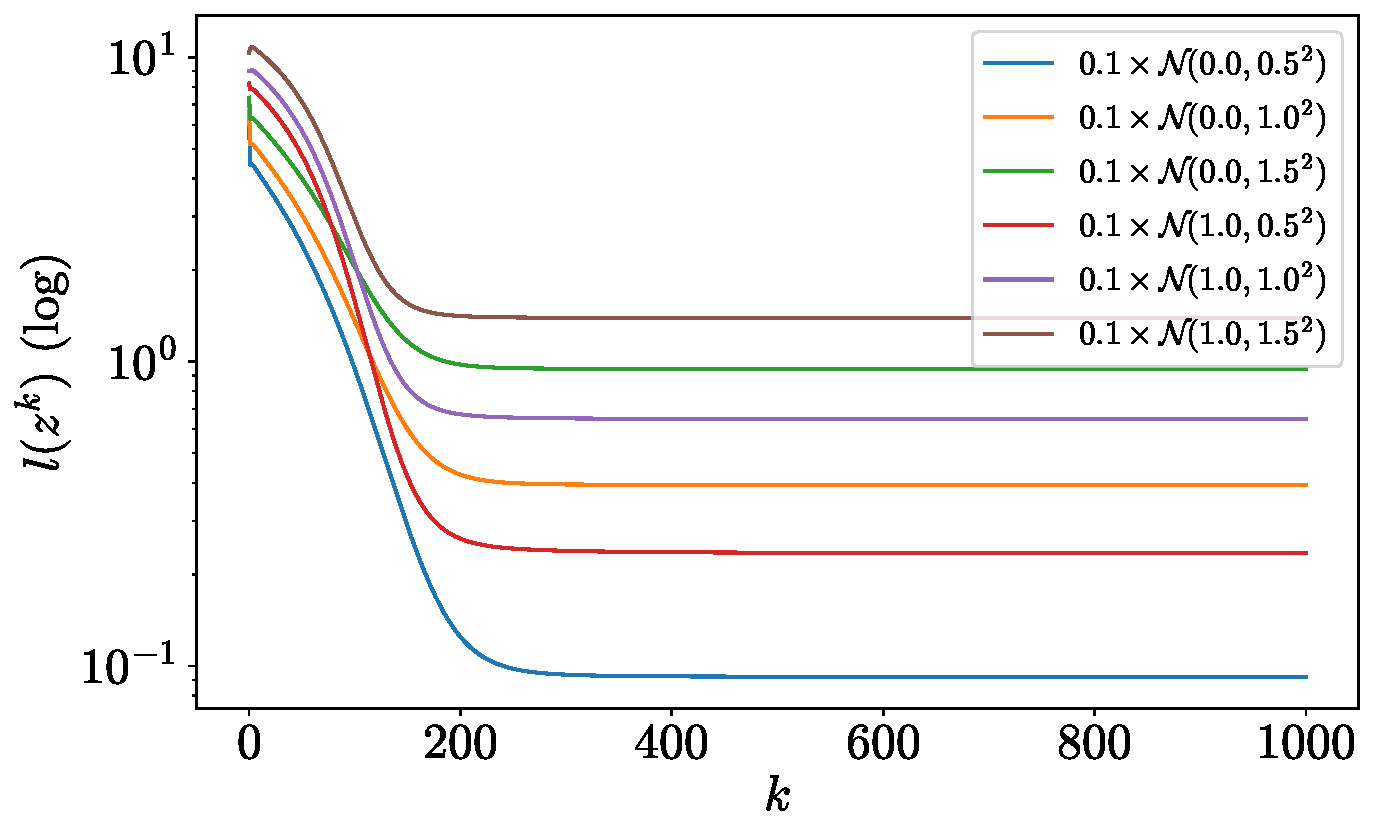
\includegraphics[width=\linewidth]{./figs/tracking/loss_gaussian_15_3_2_1000.pdf} 
            \caption{Loss evolution}
      \end{subfigure}
      \hfill
      \begin{subfigure}[t]{0.49\textwidth}
            \centering
            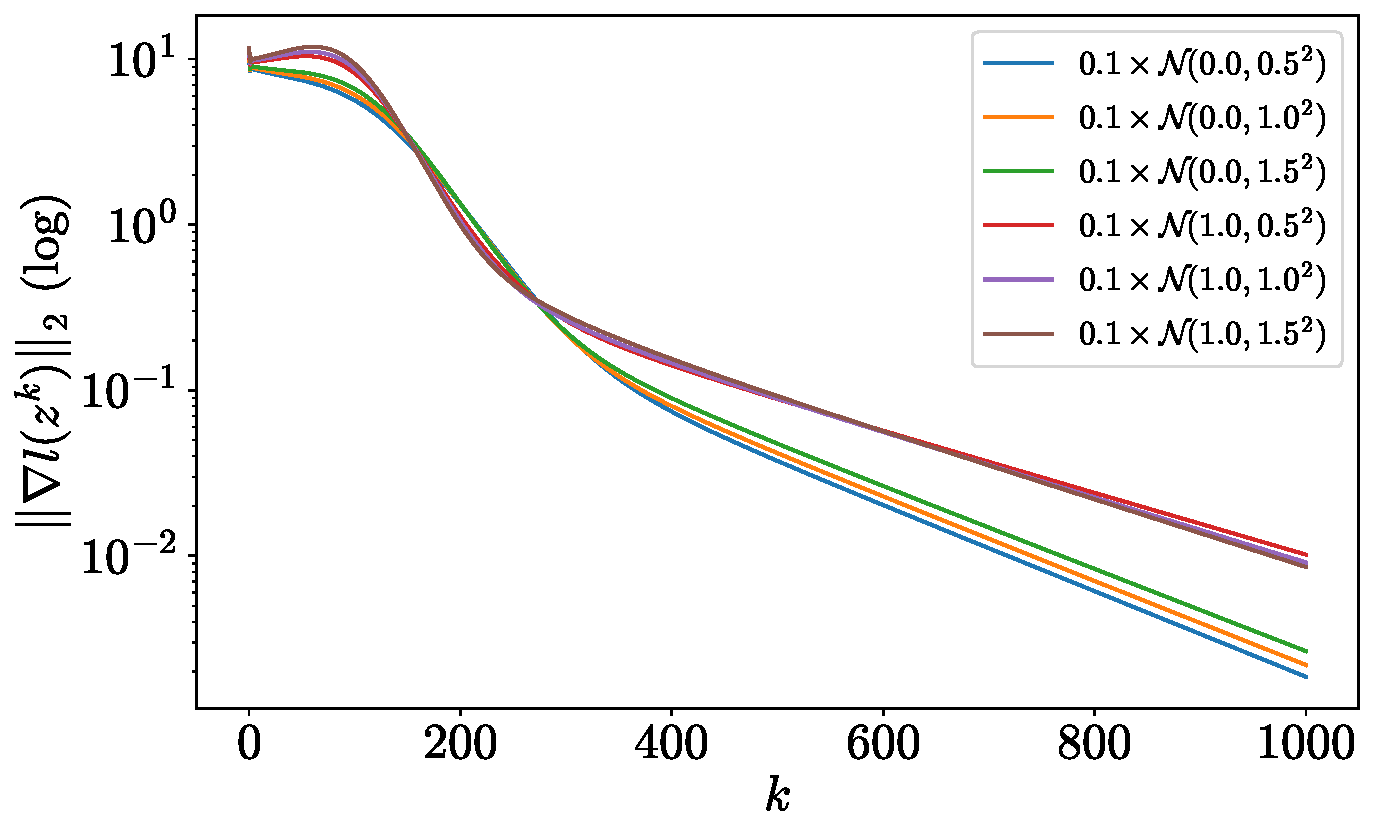
\includegraphics[width=\linewidth]{./figs/tracking/gradient_gaussian_15_3_2_1000.pdf} 
            \caption{Gradient norm evolution}
      \end{subfigure}
      \caption{Configuration with $15$ robots and $3$ targets with noise drawn from Gaussian distributions}
      \label{fig:tracking_gaussian_15_3}
\end{figure}

\begin{figure}[ht]
      \centering
      \begin{subfigure}[t]{0.49\textwidth}
            \centering
            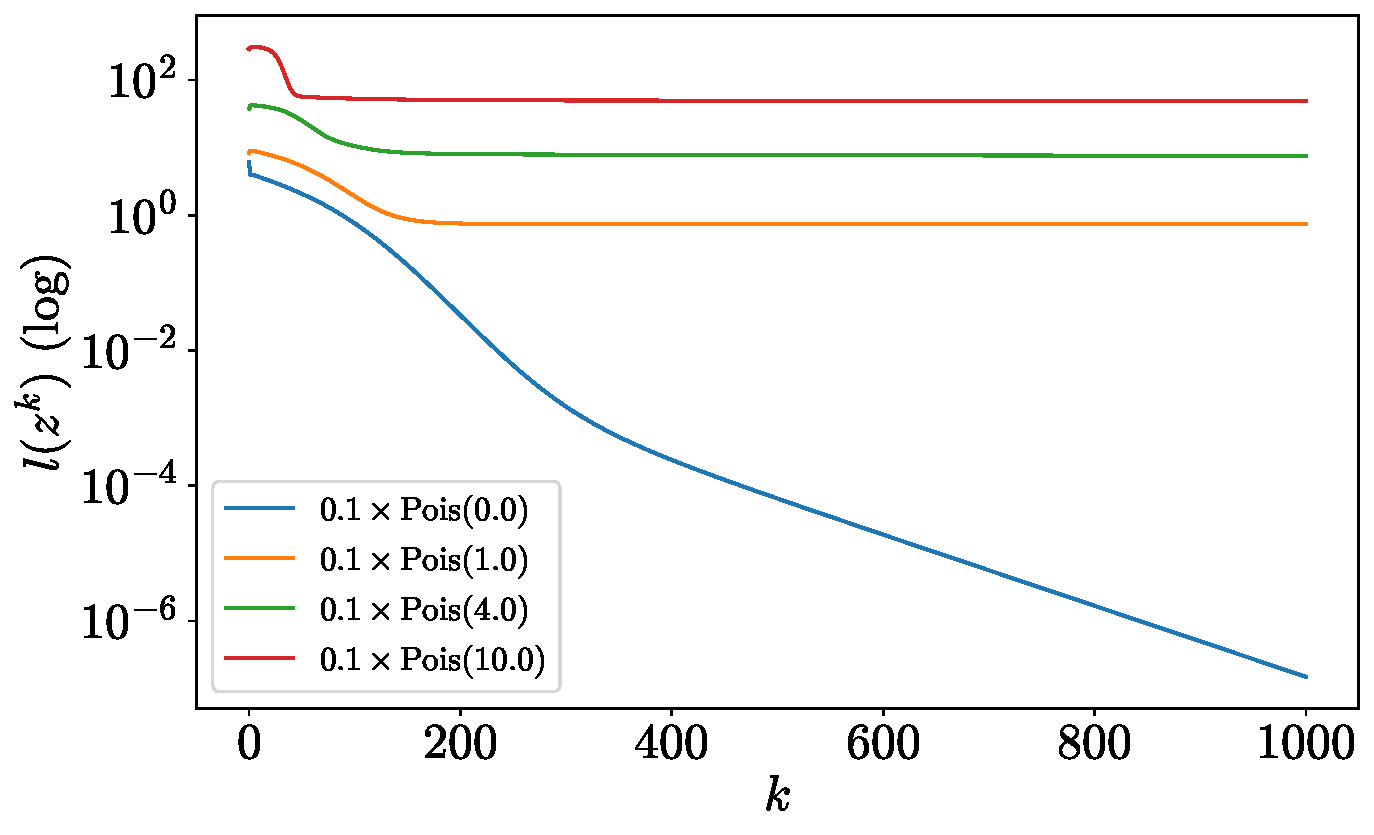
\includegraphics[width=\linewidth]{./figs/tracking/loss_poisson_15_3_2_1000.pdf} 
            \caption{Loss evolution}
      \end{subfigure}
      \hfill
      \begin{subfigure}[t]{0.49\textwidth}
            \centering
            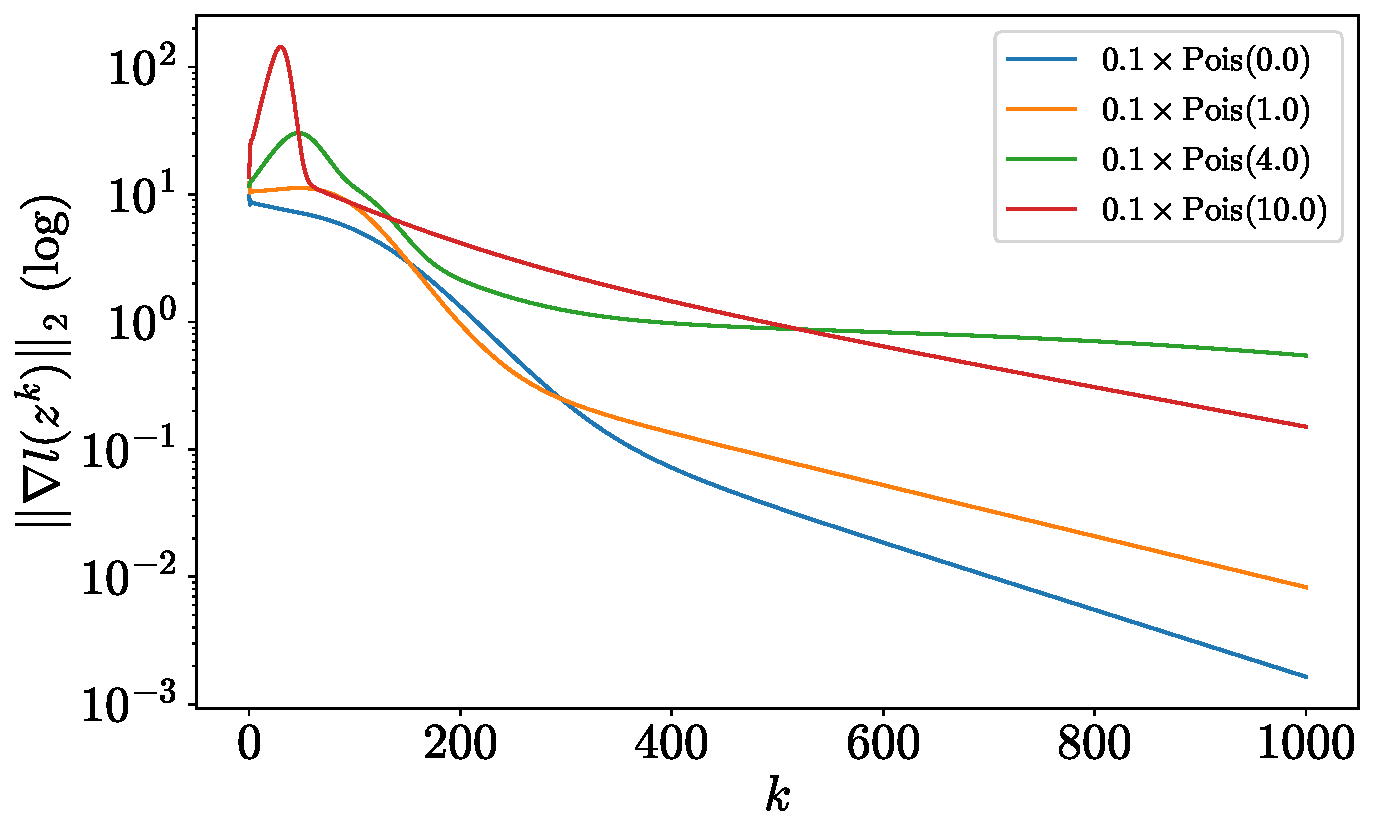
\includegraphics[width=\linewidth]{./figs/tracking/gradient_poisson_15_3_2_1000.pdf} 
            \caption{Gradient norm evolution}
      \end{subfigure}
      \caption{Configuration with $15$ robots and $3$ targets with noise drawn from Poisson distributions}
      \label{fig:tracking_poisson_15_3}
\end{figure}

\begin{figure}[ht]
      \centering
      \begin{subfigure}[t]{0.49\textwidth}
            \centering
            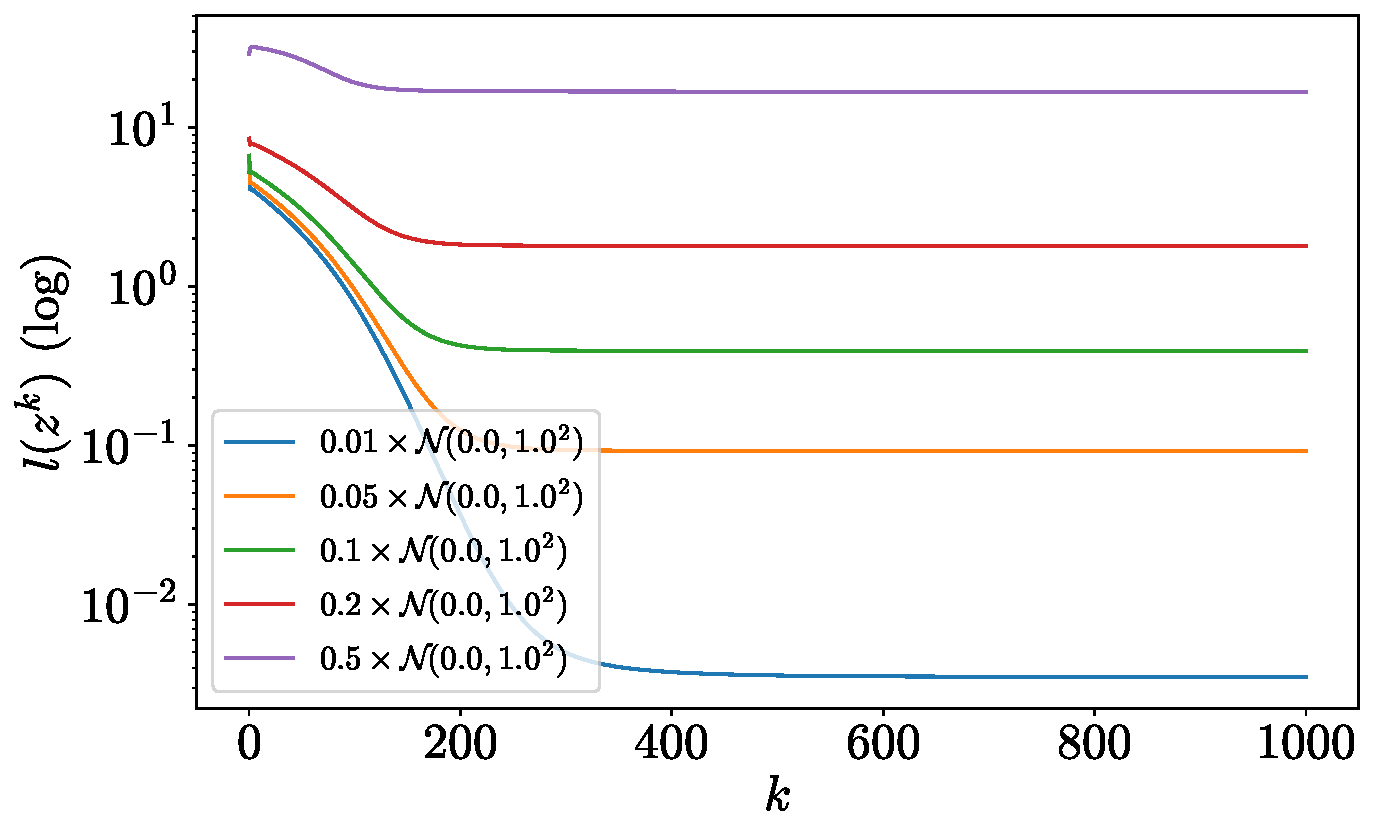
\includegraphics[width=\linewidth]{./figs/tracking/loss_rates_15_3_2_1000.pdf} 
            \caption{Loss evolution}
      \end{subfigure}
      \hfill
      \begin{subfigure}[t]{0.49\textwidth}
            \centering
            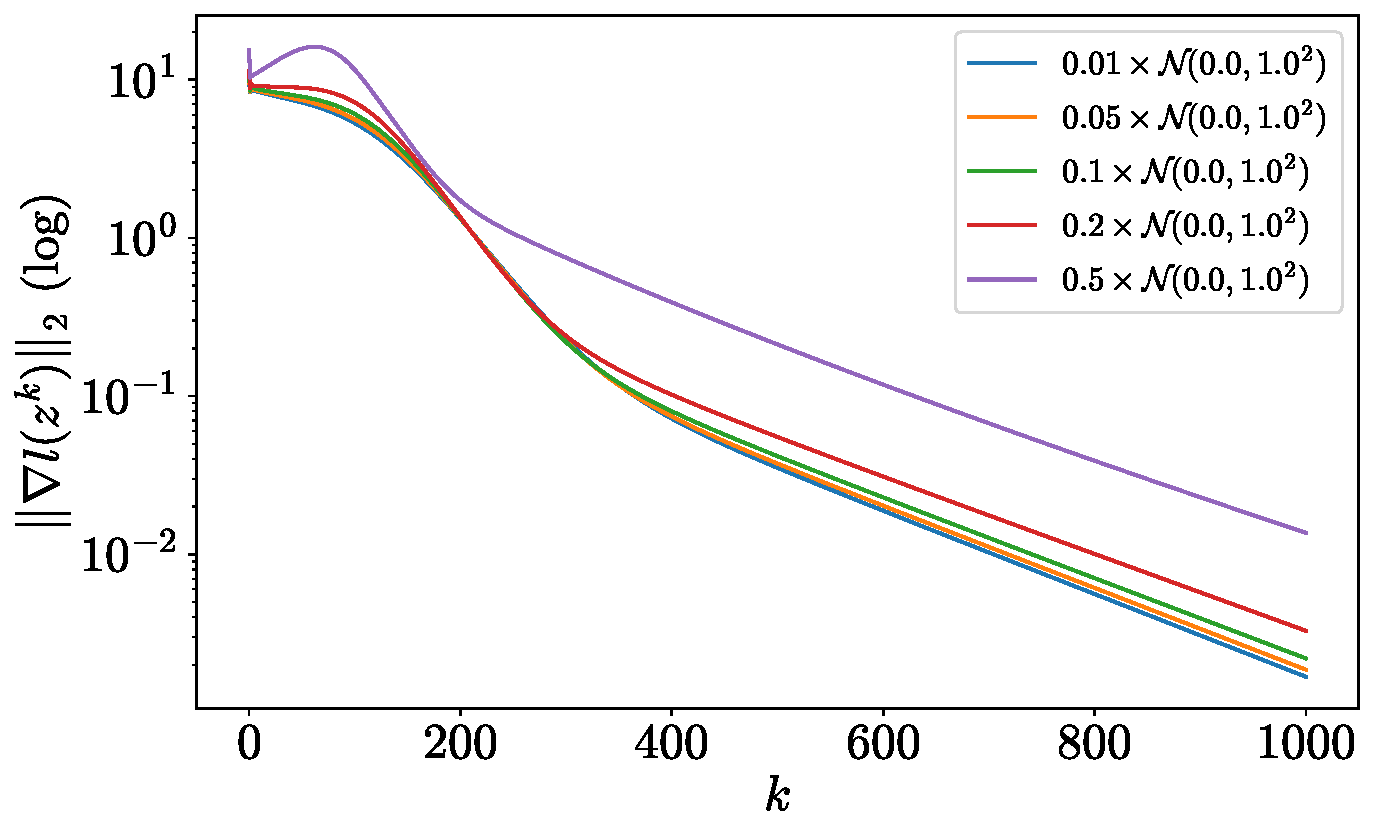
\includegraphics[width=\linewidth]{./figs/tracking/gradient_rates_15_3_2_1000.pdf} 
            \caption{Gradient norm evolution}
      \end{subfigure}
      \caption{Configuration with $15$ robots and $3$ targets with different rates of Gaussian noise}
      \label{fig:tracking_rates_15_3}
\end{figure}


\chapter{Aggregative Optimization for Multi-Robot Systems}





\chapter*{Conclusions}
\addcontentsline{toc}{chapter}{Conclusions} 



\bibliography{bibfile}{}
\bibliographystyle{plain}
\addcontentsline{toc}{chapter}{Bibliography}


\end{document}